\documentclass[10pt,a4paper]{article}
\usepackage{blindtext}
\usepackage{subcaption}
\usepackage{graphicx}
\usepackage{tikz}
\usepackage{amssymb}
\usepackage{caption}
\usepackage{amsmath}
\usepackage{circuitikz}
\usepackage{hyperref}
\usepackage{amssymb}
\usepackage{amsmath}
\usepackage{listings}

\lstset{
    inputencoding=utf8,
    extendedchars=true,
    literate={á}{{\'a}}1 {é}{{\'e}}1 {í}{{\'i}}1 {ó}{{\'o}}1 {ú}{{\'u}}1 {ñ}{{\~n}}1 {Á}{{\'A}}1 {É}{{\'E}}1 {Í}{{\'I}}1 {Ó}{{\'O}}1 {Ú}{{\'U}}1 {Ñ}{{\~N}}1
}
\input{AEDmacros}
\newcommand{\notimplies}{\;\not\!\!\!\implies}
\title{Técnicas y Diseños de Algoritmos}
\author{Tomás Agustín Hernández}
\date{}

\begin{document}
\maketitle

\begin{figure}[b]
    \centering
    \begin{tikzpicture}[remember picture,overlay]
        \node[anchor=south east, inner sep=0pt, xshift=-1cm, yshift=2cm] at (current page.south east) {
            \begin{minipage}[b]{0.5\textwidth}
                \includegraphics[width=\linewidth]{logo_uba.jpg}
                \label{fig:bottom}
            \end{minipage}
        };
    \end{tikzpicture}
\end{figure}
\newpage
\section*{Grafos}
Un grafo es una estructura de datos compuesta por \textbf{V un conjunto de vértices (nodos)} y \textbf{E un conjunto de aristas que conectan pares de vértices}. \\
Definimos un grafo como: $G = (V, E)$ donde $E \subseteq V X V$.
\[\begin{minipage}[b]{0.7\textwidth}
    \includegraphics[width=\linewidth]{assets/graph.png}
\end{minipage}\]
Nótese que tiene sentido que el conjunto de aristas E esté formado por un par $V X V$. De lo contrario no existiría una arista. \\
\textbf{Good to Know} 
\begin{itemize}
    \item Si dos vértices están conectados por una arista, entonces estos se llaman \textbf{adyacentes}.
    \item La relación entre dos vértices define a $e = (u,v) \in E$. En este caso, decimos que \textbf{e} es incidente a \textbf{u} y \textbf{v}.
    \item La cantidad de vértices la notamos con la letra \textbf{n} y la cantidad de aristas con la letra \textbf{m}.
\end{itemize}
\subsection*{¿Por qué le decimos vértices a los nodos?}
Porque los grafos tienen un fundamento mucho más matemático.
\subsection*{Self Loop (Bucle)}
En un grafo, hablamos de self loop cuando un vértice se relaciona consigo mismo.
\subsection*{Cantidad de vertices y cantidad de aristas}
Definimos la cantidad de vértices de un grafo como $\longitud{V} = n$ y la cantidad de aristas como $\longitud{E} = m$. \\
\textbf{Good to Know}: En un grafo T (árbol) \textbf{siempre} sucede que $\longitud{V} > \longitud{E}$ en una unidad. Lo veremos más adelante, pero está bueno notarlo.
\subsection*{Vecindad de un vértice}
Llamamos vecindad de un vértice v a todos los vértices adyacentes de v. \\
Formalmente, lo definimos como: $N(v) = \{u \in V : (v, u) \in E\}$ 
\[\begin{minipage}[b]{0.5\textwidth}
    \includegraphics[width=\linewidth]{assets/vecindad.png}
\end{minipage}\]
Ej.: $N(2) = \{1, 3, 7, 6\}$ \\
\textbf{Good to Know}: Se utiliza la letra N de Neighbor (vecino) en inglés.
\subsection*{Grafo Simple}
Un Grafo Simple es un grafo que no tiene más de una arista entre dos mismos nodos. Nótese que aquí no importa la relación entre ellos, sino que, no debería estar repetido el mismo par (sin importar el orden).
\begin{itemize}
    \item $E = \{(A,B), (A,B)\}$ NO es un Grafo Simple.
    \item $E = \{(A,B), (B,A)\}$ o $E = \{(B,A), (A,B)\}$ NO es un Grafo Simple.
    \item $E = \{(A,B)\}$ SÍ es un Grafo Simple.
\end{itemize}
\subsection*{Grafo no Simple}
Un Grafo no Simple es un grafo que no tiene ninguna restricción con respecto a la relación entre dos vértices (nodos). 
\begin{itemize}
    \item $E = \{(A,B), (A,B)\}$ es un Grafo no Simple.
    \item $E = \{(A,B), (B,A)\}$ o $E = \{(B,A), (A,B)\}$ es un Grafo no Simple.
    \item $E = \{(A,B)\}$ SÍ es un Grafo no Simple.
\end{itemize}
\textbf{Good to Know}: Los grafos simples, son subconjuntos de grafos no simples. Por ende, si tenemos un grafo no simple que cumple las propiedades de un grafo simple, consideramos que es un \textbf{grafo simple} al ser más restrictivo. \\
En los ejemplos anteriores, entonces, $E = \{(A,B)\}$ sería mejor considerado como Grafo Simple.
\subsection*{Multigrafo}
Un Multigrafo es un tipo de \textbf{grafo no simple} el cual puede haber más de una arista entre el mismo par de vértices. 
\[\begin{minipage}[b]{0.5\textwidth}
    \includegraphics[width=\linewidth]{assets/multigrafo.png}
\end{minipage}\]
En el gráfico anterior, se definió el siguiente multigrafo: $G = \{\textbf{(1, 2), (1, 2), (1, 2)}, (2, 3), (3, 4), (3, 2), (4, 3) ...\}$
\subsection*{Pseudografo}
Un Pseudografo es un tipo de \textbf{grafo no simple} el cual tiene la particularidad de que puede haber más de una arista entre el mismo par de vértices, y, además, los vértices pueden tener self-loops. \\
\textbf{Good to Know}: Puede haber más de un self-loop de un vértice.
\subsection*{Grado de un vértice (nodo)}
El grado de un vértice es la cantidad de conexiones que tiene un nodo. \\
Definimos formalmente al grado de un vértice como $deg(v) = \#\{e \in E : v \in e\}$ \\
\textbf{Good to Know}: deg refiere a degree. \\
\textbf{Good to Know 2}: \textbf{e} es una arista particular $e = (v, w)$.\\
\textbf{Good to Know 3}: En un grafo G, al grado mínimo lo notamos como $\delta(G)$ mientras que al grado máximo lo notamos como $\triangle(G)$
\[\begin{minipage}[b]{0.5\textwidth}
    \includegraphics[width=\linewidth]{assets/max_min_grado.png}
\end{minipage}\]
En este caso particular, tenemos que $\delta(G) = 2$ y $\triangle(G) = 4$, y, a modo de ejemplo, $deg(2) = 4$ \\
\textbf{Good to Know 4}: Por cada par de vértices, tenemos una suma de grado 2. Ej.: $\{(1,2)\}$ nos da $deg(1) + deg(2) = 2$
\subsubsection*{Grado de un vértice en un Multigrafo}
Exactamente igual que en un Grafo, pero acá hay que aclarar que como podemos tener una relación entre dos vértices más de una vez tenemos que contar cada arista. Por ejemplo, si tenemos $\{(1,2), (1,2)\}$ entonces $deg(1) = 2$.
\subsubsection*{Grado de un vértice en un Pseudografo}
Exactamente igual que en un Grafo, pero acá el self-loop cuenta 2 veces. Por ejemplo, si tenemos $\{(1,2), (1,2), (1, 1), (1, 1)\}$ entonces $deg(1) = 6$. Si en algún momento te maréas, el self-loop vale dos porque tenés el mismo número en el par.
\subsection*{Suma de los grados de los vértices}
Dado un grafo G = (V, E) la \textbf{la suma de los grados} de sus vértices es igual a 2 veces el número de aristas. Es decir, 
\[\sum_{v \in V} deg(v) = 2 \times \#\{e \in E\} = 2m\] 
Para ver acerca de cómo demostrarlo, véase \hyperref[subsubsec:suma_grados_vertices]{\textbf{anexo}} \\
\textbf{Corolario}: En un grafo, siempre hay una cantidad par de vértices que tienen grado impar. Ej.: $\{(1, 2), (2, 3)\}, deg(1) = 1, deg(2) = 2, deg(3) = 1$
\subsection*{Grafo dirigido (digrafo)}
Un grafo dirigido es un tipo de grafo (que puede ser simple o no simple) pero importa quién se relaciona con quién, es decir, el orden en que guardamos la relación. En dibujos, lo notamos con una flecha. 
\begin{itemize}
    \item $E = \{(A,B)_{\rightarrow}, (B, A)_{\leftarrow} \}$ es un grafo dirigido, esto quiere decir que $(A,B) \neq (B, A)$
\end{itemize}
\textbf{Good to Know}: A nivel estructura de datos, parece que E es igual en un Grafo Dirigido que un Grafo No Dirigido. No obstante, optamos, a nivel de notación incluir una fecha para indicar la relación entre ambos. A nivel código, deberías manejar alguna información extra para entender si es dirigido o no.
\subsubsection*{Grado de un vértice en un grafo dirigido}
En un Grafo Dirigido, el grado de un vértice se calcula como $deg(v) = indeg(v) + outdeg(v)$ \\
¿A qué nos referimos con indeg(v) y outdeg(v)? Como es un grafo dirigido, la relación entre los vértices importa. Por lo tanto, aquellas aristas entrantes al nodo v origen las agrupamos en indeg(v) mientras que aquellas aristas salientes desde el nodo v las agrupamos en outdeg(v).
\begin{itemize}
    \item $E = \{(A,B)_{\rightarrow}, (B, A)_{\leftarrow}, (A, C)_{\rightarrow} \}$ es un grafo dirigido. Siendo indeg(A) = 1, outdeg(A) = 2 $\implies deg(A) = 3$ 
\end{itemize}
\subsubsection*{Cantidad de Aristas de un grafo dirigido simple}
Como acá importa la relación los vértices pues contamos todas las aristas pues $(A,B) \neq (B,A)$ \[0 \leq |E| \leq n(n-1)\]
\subsubsection*{Cantidad de Aristas de un grafo dirigido no simple}
No hay límite, pueden ser infinitas. No hay fórmula concreta.
\subsection*{Grafo orientado}
Un grafo orientado es un digrafo que no tiene simetría en sus aristas. Es decir, si $ (u, v) \in E  \implies (v, u) \notin E$. \\
Existe un único grafo orientado donde todos sus vértices tienen grados de salida distintos. Esto es cuando el vértice 0 tiene dout(0), el vértice 1 tiene dout(1) hacia el vértice 0 y así sucesivamente.
\subsection*{Grafo no dirigido}
Un Grafo no dirigido es un grafo el cual no existe la dirección en una relación entre dos vértices.
\begin{itemize}
    \item $E = \{(A,B), (B, A) \}$ es un grafo no dirigido, esto quiere decir que $(A,B) = (B, A)$
\end{itemize}
\textbf{Good to Know}: Los grafos dirigidos o grafos no dirigidos pueden ser grafos simples o no.
\subsubsection*{Cantidad de aristas de un grafo no dirigido simple}
Como no importa la relación entre los vértices pues $(A,B) = (B,A)$, contamos solo una vez esa arista \[0 \leq |E| \leq \frac{n(n-1)}{2} = \binom{n}{2}\]
\subsubsection*{Cantidad de aristas de un grafo no dirigido no simple}
No hay límite, pueden ser infinitas. No hay fórmula concreta.
\subsubsection*{Grado de un vértice en un grafo no dirigido}
Es la misma cuenta que hacemos en un grafo dirigido, pero sin distinguir en grupos a las aristas \textbf{(porque no tienen dirección)}.
\subsection*{Grafo completo}
Llamamos Grafo Completo a un Grafo que tiene todos sus vértices están conectados entre sí. \\
Formalmente, lo notamos como $K_{n}$ donde \textbf{n} es la cantidad de vértices que tiene el grafo.
\[\begin{minipage}[b]{0.4\textwidth} 
    \includegraphics[width=\linewidth]{assets/grafo_completo.png}
\end{minipage}\]
\subsection*{Grafo complemento}
Un Grafo Complemento ($G^{C}$) es el Grafo que tiene todas las \textbf{aristas} que no estaban en G. \\
Ej.: $G = \{(1, 2), (3, 2)\}$ entonces $ G^{c} = \{(1, 3), (2, 3)\}$
\subsection*{Clausura transitiva y grafo transitivo}

La \textbf{clausura transitiva} de un grafo dirigido \(G = (V, E)\), denotada \(G^+ = (V, E^+)\), es otro grafo que contiene una arista \((u,v)\) si existe un camino desde \(u\) hasta \(v\) en el grafo original. Es decir:
\[
(u,v) \in E^+ \iff \text{existe un camino de } u \text{ a } v \text{ en } G.
\]

Un grafo se dice \textbf{transitivo} si ya contiene todas esas conexiones, es decir:
\[
G = G^+.
\]
\textbf{Ejemplo:} Si \(E = \{(1,2), (2,3)\}\), entonces su clausura transitiva es \(E^+ = \{(1,2), (2,3), (1,3)\}\).
\subsubsection*{Cantidad de aristas de un Grafo Complemento}
\[m_{\overline{G}} = \frac{n(n-1)}{2} - m\]
\textbf{Creo que es necesario que sea un Grafo simple no dirigido}
\subsection*{Recorrido}
Un recorrido es una \textbf{sucesión de vértices} y \textbf{aristas} de un grafo, tal que $e_{i}$ sea incidente a $v_{i-1}$ y $v_{i}$ para todo $i = 1...k : P = v_{0}e_{1}v_{1}e_{2}...e_{k}v_{k}$ (vértice, par de vértices, vértice, par de vértices, vértice...). \\
Ej.: $P = 1 \rightarrow (1,2) \rightarrow 2 \rightarrow (2,3) \rightarrow 3 \rightarrow (3,4) \rightarrow 4 \rightarrow (4,6) \rightarrow 6 \rightarrow (2,6) \rightarrow 2 ...$ \\
Es decir, el nodo anterior (si hay) debe estar en la siguiente arista en alguna de las posiciones.
\subsection*{Camino}
Un camino es un recorrido \textbf{que no pasa dos veces} por el mismo vértice. \\
Ej.: $P = 1 \rightarrow 2 \rightarrow 3 \rightarrow 4 \rightarrow 5 \rightarrow 6 \rightarrow 7 \rightarrow 8 \rightarrow 9$
\[\begin{minipage}[b]{0.4\textwidth}
    \includegraphics[width=\linewidth]{assets/camino.png}
\end{minipage}\]
\subsection*{Sección (subconjunto/parte de un recorrido)}
Una sección es un tramo del recorrido P, se nota $P_{v_{i}}{v_{j}}$. Nótese que P es el recorrido, y los subíndices es aquello que acota al mismo. \\
Ej.: $P_{2,6} = 2 \rightarrow 3 \rightarrow 4 \rightarrow 6$. En este ejemplo, $v_{i} = 2$ y $v_{j} = 6$.
\[\begin{minipage}[b]{0.6\textwidth}
    \includegraphics[width=\linewidth]{assets/sección.png}
\end{minipage}\]
\textbf{Good to Know}
\begin{itemize}
    \item Una sección es un subconjunto de un recorrido P.
\end{itemize}
\subsection*{Circuito}
Un circuito es un recorrido que empieza y termina en el mismo vértice, se nota $P_{v_{i}}{v_{j}}$ \\
Ej.: $P_{1,1} = 1 \rightarrow 2 \rightarrow 3 \rightarrow 4 \rightarrow 6 \rightarrow 2 \rightarrow 1$
\[\begin{minipage}[b]{0.6\textwidth}
    \includegraphics[width=\linewidth]{assets/circuito.png}
\end{minipage}\]
\textbf{Good to Know}:
\begin{itemize}
    \item Un circuito es un tipo de recorrido. 
    \item Un circuito es opuesto a un camino. Porque un camino no tiene repetidos.
\end{itemize}
\subsection*{Ciclo (o circuito simple)}
Un ciclo o circuito simple es un circuito (de tres o más vértices) que no repite vértices, se nota $P_{v_{i}}{v_{j}}$.
Ej.: $P_{1,1} = 1 \rightarrow 2 \rightarrow 3 \rightarrow 4 \rightarrow 6 \rightarrow 7 \rightarrow 8 \rightarrow 9 \rightarrow 1$
\[\begin{minipage}[b]{0.6\textwidth}
    \includegraphics[width=\linewidth]{assets/ciclo.png}
\end{minipage}\]
\subsubsection*{Longitud}
La longitud de un recorrido P denotada l(P), es la \textbf{cantidad de aristas} que tiene. \\
$Ej.: P = 1 \rightarrow 2 \rightarrow 3 \rightarrow 4 \rightarrow 6 \rightarrow 2 \rightarrow 7$ donde $l(P) = 6$
\textbf{Good to Know}: Esta definición es muy importante, porque tranquilamente podría haber dos recorridos diferentes entre cada par de vértices.
\subsubsection*{Distancia entre dos vértices}
La distancia entre dos vértices u y v se define como la \textbf{longitud del recorrido más corto} entre u y v. Se denota $d(u,v)$ 
\[\begin{minipage}[b]{0.7\textwidth}
    \includegraphics[width=\linewidth]{assets/distancia.png}
\end{minipage}\]
\textbf{Good to Know} 
\begin{itemize}
    \item Precondiciones
    \begin{itemize}
        \item Tener dos vectores: u y v que pertenezcan a un grafo G.
        \item Tener uno o más recorridos, que incluyan los nodos de G.
    \end{itemize}
    \item Postcondiciones
    \begin{itemize}
        \item d(u,v) es el recorrido más corto desde u a v.
        \item Si $u=v \iff d(u,v) = 0$
        \item Si no existe un recorrido entre u y v entonces $d(u,v) = \infty$
    \end{itemize}
\end{itemize}
Véase \hyperref[subsubsec:distancia_demostracion]{\textbf{anexo}} para ver como demostrarlo por absurdo.
\subsubsection*{Camino en un grafo dirigido}
Importa quién se relaciona con quien. Ej.: $E = \{(A, B)_{\rightarrow}, (B, C)_{\rightarrow}\}$
\subsubsection*{Camino en un Grafo no Dirigido}
No importa quién se relaciona con quien. Ej.: $E = \{(A, B), (B, C)\}$. El camino podría ser en cualquier sentido. 
\subsection*{Subgrafo}
Sea $G = (V_{G}, E_{G})$ y $H = (V_{H}, E_{H})$ 
\subsubsection*{Subgrafo (base)}
H es un subgrafo de G si todos los vértices y aristas de H están en G. \\
Esto quiere decir que con que no haya aristas (conexiones entre vértices) o vértices que no estén en G, H es un subgrafo de G.
\[\begin{minipage}[b]{0.8\textwidth}
    \includegraphics[width=\linewidth]{assets/subgrafo_base.png}
\end{minipage}\]
\textbf{A partir de acá, los demás subgrafos cumplen mínimamente estas condiciones}
\subsubsection*{Subgrafo propio}
H es un subgrafo propio de G si todos los vértices y aristas de H están en G siempre y cuando \textbf{no sea la totalidad}. Es decir, no debe suceder que sea exactamente $H = G$.
\[\begin{minipage}[b]{0.8\textwidth}
    \includegraphics[width=\linewidth]{assets/subgrafo_propio.png}
\end{minipage}\]
\subsubsection*{Subgrafo generador}
H es un subgrafo generador de G si H \textbf{tiene exactamente los mismos vértices} que G. 
\[\begin{minipage}[b]{0.8\textwidth}
    \includegraphics[width=\linewidth]{assets/subgrafo_generador.png}
\end{minipage}\]
\textbf{Un subgrafo generador es más fuerte que un subgrafo propio porque nos hacen usar todos los nodos pero conectarlos como queramos (siempre y cuando esas conexiones existan en el grafo original). Un subgrafo propio solo tiene una condición, no ser igual al grafo original.}
\subsubsection*{Subgrafo inducido}
H es un subgrafo inducido de G si todos los nodos que están en H tienen todas las aristas de G que contienen exactamente a los nodos de H. 
Ej.: $G = ((1, 2, 3), \{(1,3), (1,2)\})$ si $H = (1,2)$ entonces está obligado a tener las aristas que contengan exactamente a los elementos 1 y 2. Por lo tanto serían: $\{1, 2\}$ 
\subsection*{Grafo conexo}
Un Grafo Conexo es un grafo el cual existe un \textbf{camino} que conecta todos los vértices entre sí. 
\begin{itemize}
    \item $E = \{(A,B)_{\rightarrow}, (B, C)_{\rightarrow}, \}$ es un grafo conexo.
    \item $E = \{(A, B)_{\rightarrow}, (C, D)_{\rightarrow}\}$ no es un grafo conexo.
\end{itemize}
\subsubsection*{Componente conexa}
Una componente conexa es un subgrafo.
\[\begin{minipage}[b]{0.9\textwidth}
    \includegraphics[width=\linewidth]{assets/componente_conexa.png}
\end{minipage}\]
Normalmente se consiguen cuando desconectás alguna arista de un grafo conexo. Entonces, te quedan subgrafos. La cantidad de subgrafitos son los componentes conexos.
\subsubsection*{Grafo fuertemente conexo}
Un Grafo fuertemente conexo es un grafo dirigido y conexo. Es decir, si desde todos los nodos puedo pasar por todos los demás siguiendo la dirección. 
\[\begin{minipage}[b]{0.9\textwidth}
    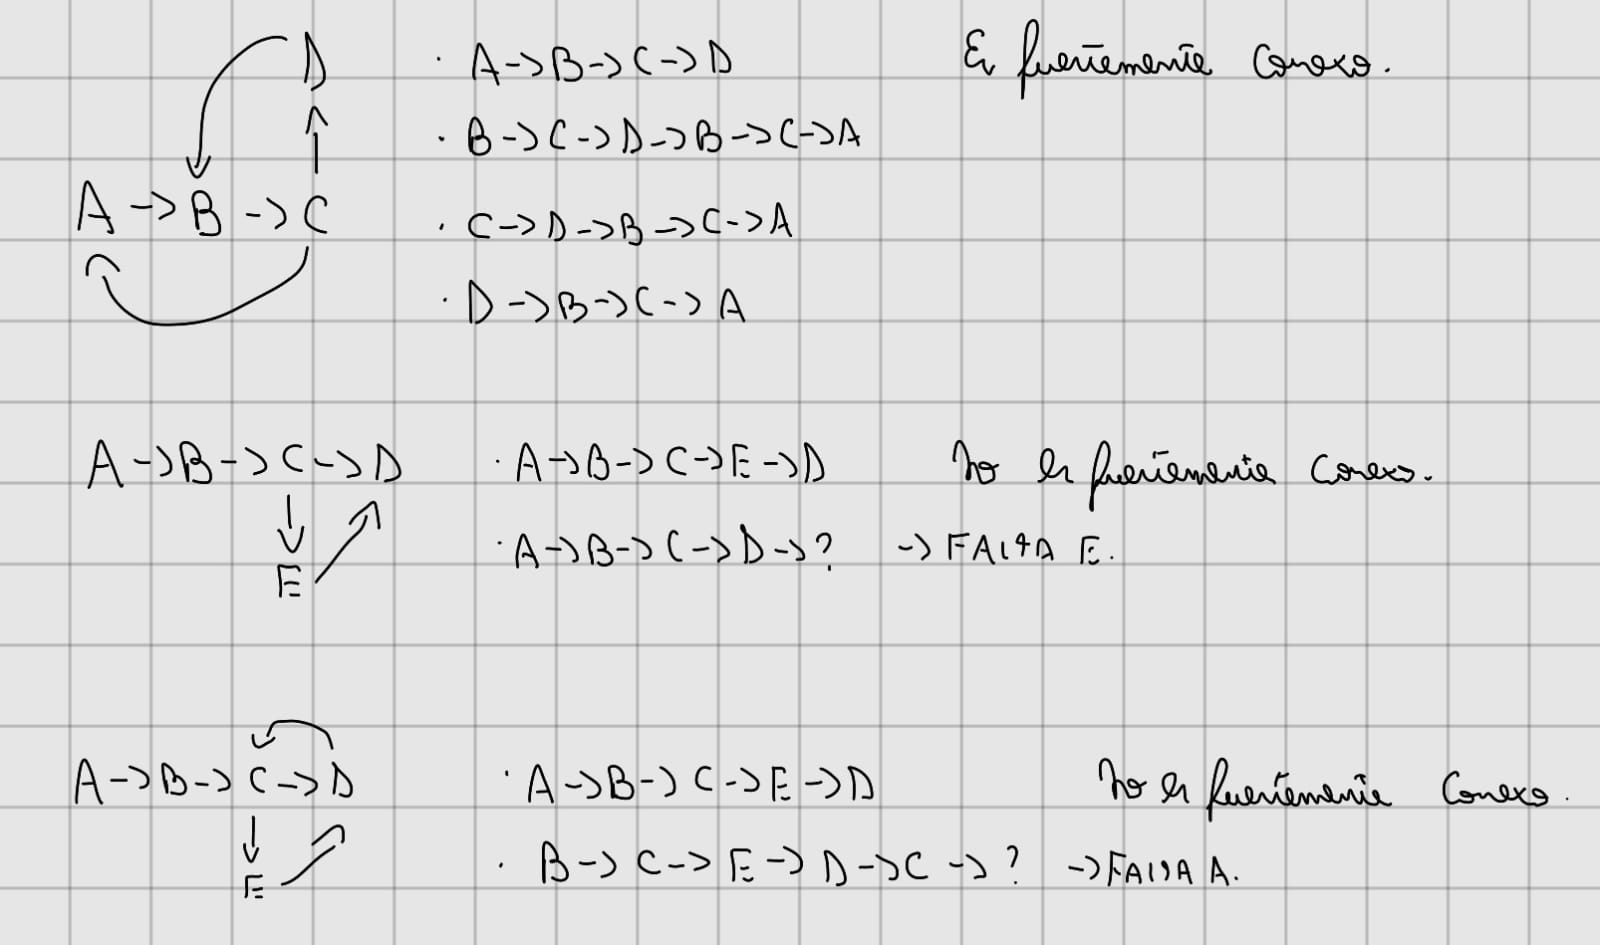
\includegraphics[width=\linewidth]{assets/fuertemente_conexo.jpg}
\end{minipage}\]

\subsection*{Árboles}
\subsubsection*{Base}
Es un grafo conexo, sin ciclos (circuitos simples).
\[\begin{minipage}[b]{0.6\textwidth}
    \includegraphics[width=\linewidth]{assets/arbol_grafo.png}
\end{minipage}\]
\subsubsection*{Quitar Arista}
Si quitamos una arista cualquiera de un árbol, tenemos dos subgrafos conexos. Esto porque inicialmente un árbol no tiene ninguna componente suelta en el aire. 
\[\begin{minipage}[b]{0.6\textwidth}
    \includegraphics[width=\linewidth]{assets/arbol_quitar_arista.png}
\end{minipage}\]
\subsubsection*{Agregar Arista}
Si agrego una arista cualquiera se forma un ciclo (circuito simple).
\[\begin{minipage}[b]{0.8\textwidth}
    \includegraphics[width=\linewidth]{assets/arbol_agregar_arista.png}
\end{minipage}\]
\subsection*{Árbol T}
Es un árbol que cumple con las siguientes propiedades
\begin{itemize}
    \item Es conexo.
    \item No tiene ciclos. 
\end{itemize}
\subsection*{Grafo Pesado}
Definimos un Grafo Pesado G como $G = (V, E, W)$ donde W es una función que recibe dos vértices y devuelve el peso. \\
Ahora, en cada arista almacenamos ambos vértices y el resultado del peso. 
\[E_{i} = (v_{i}, v_{j}, w(v_{i},v_{j}))\]
\textbf{Good to Know}: En inglés, decimos \textbf{weighted graphs} mientras que en español también los conocemos por ser \textbf{grafos ponderados}.
\subsubsection*{Camino en Grafo Pesado}
En grafos pesados, el camino más corto entre dos nodos u y v es el que tiene la menor suma de pesos en sus aristas, sin importar cuántas aristas lo componen.
\subsubsection*{Ciclos Negativos en Grafos Pesados}
Un grafo pesado G tiene un ciclo negativo si la \textbf{suma de los pesos de las aristas} es negativa. 
\begin{lstlisting}
    A -> B (peso 2)
    B -> C (peso -4)
    C -> A (peso 1)

    Suma total del ciclo: 2 + (-4) + 1 = -1
\end{lstlisting}
Entonces, $ A \rightarrow B \rightarrow C \rightarrow A$ es un ciclo negativo.
\subsection*{Grafo Acíclico Dirigido (DAG)}
Un Grafo Acíclico Dirigido es un grafo dirigido que no tiene ciclos. Es decir, no existe ningún vértice que es capaz de empezar y terminar un recorrido. \\
Ej.: Una Single Linked List es un caso particular de un DAG. \\
Script de Python para ver si un grafo dirigido es acíclico 
\[\begin{minipage}[b]{1\textwidth}
    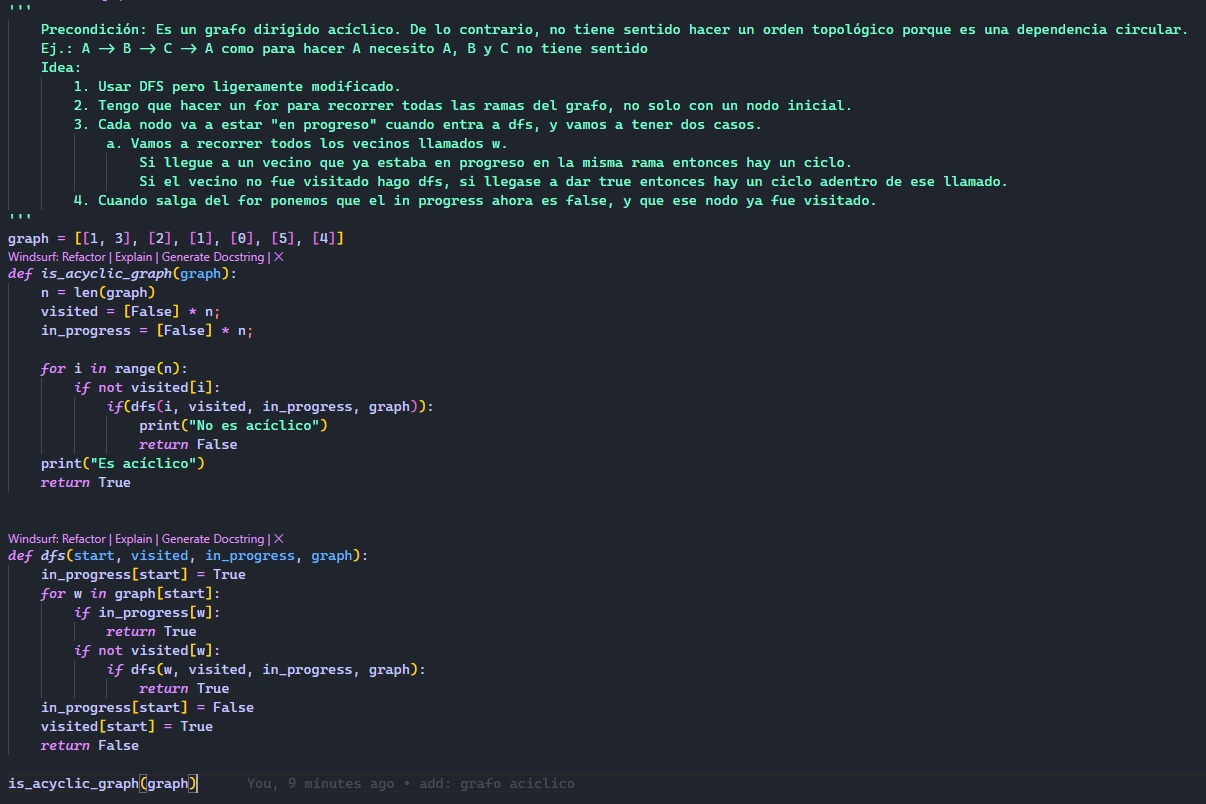
\includegraphics[width=\linewidth]{assets/acyclic_graph_py.jpg}
\end{minipage}\]
\subsection*{Orden Topológico}
\begin{itemize}
    \item Es una lista de nodos ordenados de forma que, si existe una arista $u \rightarrow v$, entonces $u$ aparece antes que $v$ en la lista.
    \item Es útil para resolver problemas donde ciertas tareas deben ejecutarse antes que otras, como en compiladores, donde un archivo puede depender de otros.
    \item Este orden no es único. ¿Por qué? Porque si hay nodos que no dependen de nadie, su posición relativa puede variar sin romper la condición del orden.
    \item \textbf{Ejemplo}: Dado el grafo con aristas $A \rightarrow C$ y $B \rightarrow C$, hay dos órdenes topológicos posibles: 
    \[
    A, B, C \quad \text{o} \quad B, A, C
    \]
    \item Esto se debe a que tanto $A$ como $B$ no dependen de ningún otro nodo, por lo que pueden aparecer en cualquier orden. El nodo $C$ depende de ambos, así que debe aparecer después de $A$ y $B$.
\end{itemize}
Véase \hyperref[subsubsec:topological_sort]{\textbf{Topological Sort}} para un caso de uso real con DFS y ejemplos. 
\subsection*{Grafo Bipartito}
Dado un grafo $G = (V, E)$, G es bipartito si
\begin{itemize}
    \item Existe $V_{1}$ y $V_{2}$ tal que $V_{1} \cup V_{2} = V$
    \item $V_{1} \cap V_{2} = \emptyset$
    \item $e = (u,v) \in E, u \in V_{1}, v \in V_{2}$. Esto significa que el vértice de $V_{1}$ se relaciona con el de $V_{2}$ o en el otro sentido. 
    \item La única restricción es que no podés conectar un vértice de $V_{1}$ con otro de $V_{1}$ ni tampoco uno de $V_{2}$ con otro de $V_{2}$
\end{itemize}
\textbf{Importante}
\begin{itemize}
    \item Un grafo es bipartito, $V = (V_{1}, V_{2}) \iff$ no tiene ciclos de longitud impar.
    \begin{itemize}
        \item Imaginemos que tenemos 3 vértices conectados entre sí. Va a suceder, sí o sí que al menos, dos vértices van a pertenecer al mismo conjunto. Eso ya rompe la bipartición. 
        \item Para poder encontrar si un grafo es bipartito es usar DFS, ir colocreando desde un nodo raíz con sus vecinos adyacentes de color diferente alternando y si nos encontramos dos colores iguales continuos entonces no es bipartito.
    \end{itemize}
    \item Un grafo es bipartito $\iff$ todas sus c.c. lo son 
    \item Un grafo no tiene ciclos impares $\iff$ cada una de sus c.c. no tienen ciclos impares.
\end{itemize}
\subsection*{Grafo Bipartito Completo}
Lo mismo que un Grafo Bipartito pero acá todos los vértices de $V_{1}$ están conectados con los de $V_{2}$ y viceversa. \\
Básicamente, el producto cartesiano.
\subsection*{Isomorfismo de Grafos}
Dados  $G = (V, E)$ y $G' = (V', E')$. $G$ y $G'$ son isomorfos si existe una función biyectiva $f: V \rightarrow V$ tal que $\forall u,v \in V$ 
\[(u,v) \in E \iff (f(u), f(v)) \in E'\]
Es decir, \textbf{si parto desde E y agarro el par que está en una arista, puedo poner cada componente en una función f y me lo transforma en una arista que está en E'}. \\
Lo mismo con el caso opuesto. \\
\textbf{Good to Know}: En nuestro caso, si G y G' son isomorfos los vamos a notar como $G = G'$ porque son lo mismo pero cambian la forma en que se nombran los nodos y el orden de las aristas.
\subsubsection*{Propiedades}
Si dos grafos $G = (V,E)$ y $G' = (V', E')$ son isomorfos entonces
\begin{itemize}
    \item Tienen el mismo número de vértices (sí, porque en la biyectividad se cumple la inyectividad y la sobreyectividad).
    \item Tienen el mismo número de aristas (sí, porque cada una debería traducirse a una única específica, de lo contrario no sería inyectiva).
    \item Para todo $k$, $1 \le k \le n-1$, tienen el mismo número de vértices de grado k (la misma distribución de grado).
    \item Tienen la misma cantidad de componentes conexas.
    \item Para todo k, $1 \le k \le n-1$, tienen el mismo número de caminos simples de longitud k.
\end{itemize}
\[\begin{minipage}[b]{0.8\textwidth}
    \includegraphics[width=\linewidth]{assets/isomorfos.png}
\end{minipage}\]
\subsection*{Representación de grafos}
\textbf{Good to Know}: Si busca uso de grafos en la práctica, y cómo representarlos véase \hyperref[subsec:representacion_grafos_practica]{\textbf{anexo}}.
\textbf{Good to Know}: En las diapositivas se usa la $d$ para representar tanto como el grado de un vértice o la distancia entre dos vértices. Acá, optamos por usar $deg$ para el grado y $d$ para distancia entre dos vértices.
\subsubsection*{Lista de Adyacencia}
Es la más común y la más eficiente. \\
Es una lista de listas, donde cada lista corresponde al vértice y las aristas con las que se conecta se representa con una lista de diccionarios. 
\[\begin{minipage}[b]{0.8\textwidth}
    \includegraphics[width=\linewidth]{assets/adj_list.png}
\end{minipage}\]
\subsubsection*{Matriz de Adyacencia}
Cada número está representado por el índice en donde está. Vale 1 \textbf{(o el valor de peso de la arista)} si existe la arista y 0 si no. \\
La cantidad de filas y columnas es igual a la cantidad de nodos que hay, es por eso que espacialmente cuesta $O(n^{2})$
\[\begin{minipage}[b]{0.8\textwidth}
    \includegraphics[width=\linewidth]{assets/matriz_ady.png}
\end{minipage}\]
Ej.: El nodo 3 (fila 3), está relacionado con todos los nodos que están en la columna 3. En el dibujo, el nodo 3 está relacionado con el 2 y con el 4. Por eso, $a_{3, 2}$ = 1 y $a_{3, 4}$. 
\[\begin{minipage}[b]{0.8\textwidth}
    \includegraphics[width=\linewidth]{assets/adj_matrix.png}
\end{minipage}\]
\textbf{Good to Know}
\begin{itemize}
    \item En el dibujo vemos que empieza todo desde el índice 1 pero en realidad empezamos desde el 0. 
    \item \textbf{Lo que todavía no entiendo es, qué pasaría si los nodos guardan información compleja, como elijo cual va en el índice 0, cual en el 1, etc.} 
    \item La matriz es simétrica si el grafo es no dirigido. Es decir, ver desde fila/columna o columna/fila es lo mismo. 
\end{itemize}
Esta forma de trabajar con grafos es \textbf{súper ineficiente}. \\
¿Esto significa que nunca usaremos matrices? ¡No! Véase \hyperref[subsec:representacion_grafos_practica]{\textbf{anexo}} para ver casos de uso.
\subsubsection*{Algunas propiedades útiles (solo grafos no dirigidos)}
\begin{itemize}
    \item 1. La suma de los elementos de la fila i (o columna j) es igual a $deg(u_{i})$, es decir: \textbf{$\sum_{i=0}^{j} a[i][0] = \sum_{j=0}^{i} a[j][0]$}
    \item 2. Los elementos de la diagonal principal de $A^{2}$ indican los grados de los vértices $a^{2}_{ii} = deg(u_{i})$. \textbf{Nota}: usa ${ii}$ porque hay misma cantidad de filas que de columnas, de lo contrario, se podría decir ${ij}$ con $i=j$. Esto es más que nada para hablar de los índices de la diagonal principal de una matriz.
\end{itemize}
1. Nótese que en la columna $a_{i, ultColumna + 1}$ o en la fila $a_{ultFila + 1, j}$ se encuentran las sumas de esa fila o columna.
\[\begin{minipage}[b]{0.9\textwidth}
    \includegraphics[width=\linewidth]{assets/suma_matriz_ady.png}
\end{minipage}\]
2. Nótese que ahora lo que estaban en la fila / columna extra, ahora se pasaron al $a_{ii}$ (o $a_{ij}$ con $i=j$)  correspondiente.
\[\begin{minipage}[b]{0.6\textwidth}
    \includegraphics[width=\linewidth]{assets/diagonal_principal_ady.png}
\end{minipage}\]
\subsection*{Matriz de Adyacencia con Grafos Dirigidos}
\begin{itemize}
    \item La matriz de adyacencia de un grafo dirigido NO es simétrica como sí pasaba con un grafo común.
    \item G = (V, E) donde E es un conjunto de pares ordenados. Esto significa que el \textbf{orden de los elementos del par} importan.
    \item $e=(u,v)$ también se llama \textbf{arco}. A $u$ se le llama \textbf{cola} y a $v$ se le llama \textbf{cabeza}. (medio raro, pero bueno).
    \item Los digrafos tienen grados de entrada $(deg_{in})$ y grados de salida $(deg_{out})$
    \item El grafo subyacente $(G^{s})$ es el que resulta de remover las direcciones.
    \item La suma de los elementos de la fila i es igual a $d_{OUT(u_{i})}$.
    \item La suma de los elementos de la columna j es igual a $d_{IN(u_{j})}$
\end{itemize} 
\section*{Algoritmos de Búsqueda en Grafos}
Recorrer grafos nos da mucha información acerca de su estructura.
\subsection*{BFS (Técnica Greedy)}
Breadth-First Search o mejor conocido como BFS es un algoritmo de búsqueda para grafos. \\
Casos de uso: 
\begin{itemize}
    \item Vale para cualquier tipo de grafo $(*^{1})$
    \item \textbf{Sirve} para buscar el \textbf{camino mínimo} de un nodo a otro. 
    \item Se usa para asegurarnos que siempre pasamos por todos los nodos del mismo nivel antes de pasar a otro. 
    \item Explora el grafo o árbol nivel a nivel, primero horizontalmente y luego verticalmente. Es decir, primero agarra todos los vecinos, después del primer vecino baja al siguiente nivel, después del segundo vecino baja al siguiente nivel y así sucesivamente. 
    \item A nivel estructura de datos se implementa con una \textbf{queue} (FIFO).
    \item Se almacena en una lista los nodos visitados para no repetirlos. Es decir, que antes de pasar por uno hay que chequear si ya está.
\end{itemize}
\textbf{Good to Know $(*^{1})$}: Si usamos BFS en un Grafo G pesado \textbf{NO NOS GARANTIZA} que sea el camino mínimo, porque BFS calcula el camino con menor cantidad de aristas, y no con menor peso. 
\subsubsection*{Complejidad temporal de BFS}
La complejidad temporal de BFS es $O(\longitud{V} + \longitud{E})$. 
\subsection*{DFS}
Depth-First Search o mejor conocido como DFS es un algoritmo de búsqueda para grafos. 
\begin{itemize}
    \item Explora todos los nodos a profundidad, primero verticalmente y luego horizontalmente.
    \item A nivel estructura de datos se implementa con un \textbf{stack} (LIFO).
    \item \textbf{NO sirve} para buscar el camino más corto de un nodo al otro. Esto es debido a que ingresa a las ramas en profundidad.
    \item Vale para cualquier tipo de grafo $(*^{2})$
\end{itemize}
Un ejemplo claro de DFS sería buscar la altura de un árbol porque tendrías que buscar la rama más larga. \\
\textbf{Good to Know $(*^{2})$}: Si usamos DFS en un Grafo G pesado \textbf{NO NOS GARANTIZA} que sea el camino mínimo, porque DFS calcula el camino con menor cantidad de aristas, y no con menor peso. 
\subsubsection*{Complejidad temporal de DFS}
La complejidad temporal de DFS es $O(\longitud{V} + \longitud{E})$. \\
\textbf{Good to Know}: Pese a que se implementa recursivamente o iterativamente, la complejidad podría parecer que es $O(\longitud{V} * \longitud{E})$ pero es $O(\longitud{V} + \longitud{E})$ porque cada arista se visita una sola vez.
\subsubsection*{Casos de uso de DFS}
\begin{itemize}
    \item Recorrer todos los vértices.
    \item Detectar si un grafo es bipartito.
    \item Detectar si el grafo tiene ciclos. 
    \item Detectar si un grafo es conexo
    \begin{itemize}
        \item Si el grafo es dirigido no es tan sencillo con DFS porque se usan otras cosas.
        \item Si el grafo es NO dirigido si es sencillo de saberlo. 
    \end{itemize}
    \item Hallar componentes conexas.
    \item Construir un árbol DFS. 
    \item Buscar si hay un camino entre dos vértices.
    \item En grafos DAG nos da el orden topológico. Se usa para marcar el post orden y luego se invierte ese orden. 
\end{itemize}
¿Cuándo usar DFS? 
\begin{itemize}
    \item Cuando querés explorar una componente rápidamente.
    \item No te interesa la distancia mínima (para eso usá BFS).
    \item El grafo es grande pero poco denso. 
    \item Estás haciendo un análisis estructural.
\end{itemize}
\textbf{Importante}: Si un grafo G es conexo basta con ejecutar DFS con un único nodo inicial.
\[\begin{minipage}[b]{0.8\textwidth}
    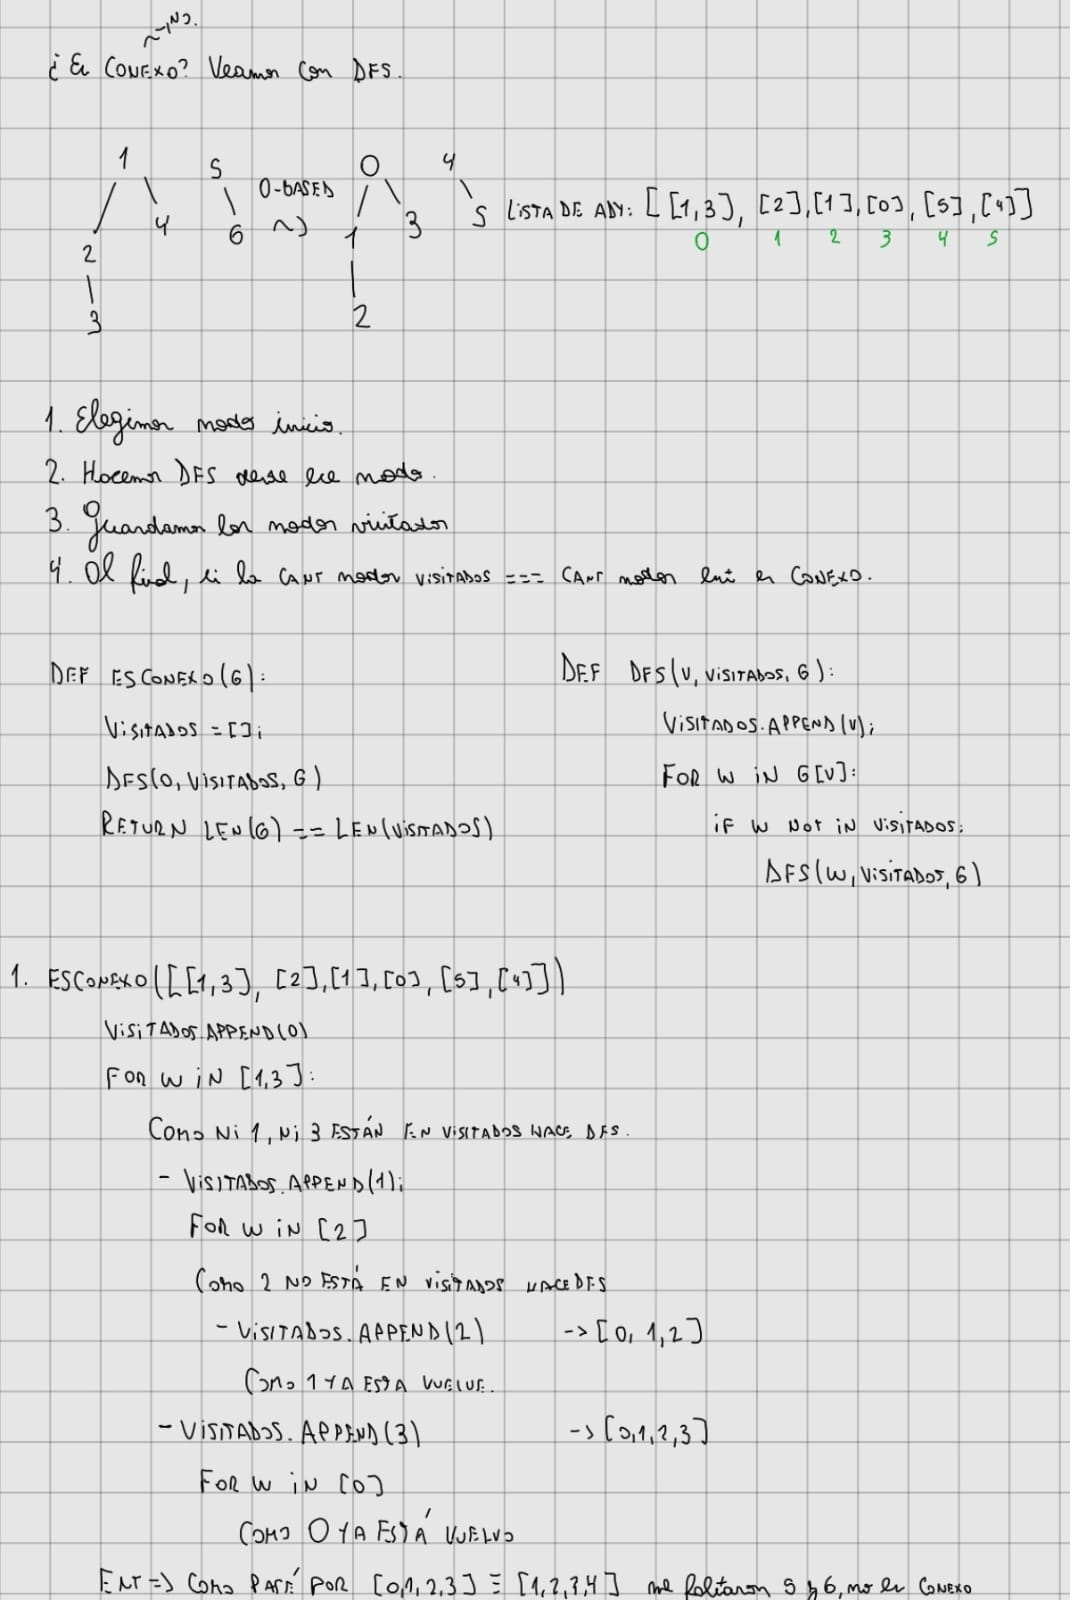
\includegraphics[width=\linewidth]{assets/dfs_py.jpg}
\end{minipage}\]
\subsection*{Algoritmos de Búsqueda de Camino Mínimo (Grafos Pesados)}
\begin{itemize}
    \item Single-Source-Shortest-Paths: Para encontrar el camino mínimo desde un nodo particular a todos los demás nodos. Resuelve \textbf{uno a muchos}.
    \begin{itemize}
        \item Dijkstra, Bellman-Ford
    \end{itemize}
    \item All-Pairs-Shortest-Paths: Para encontrar el camino mínimo desde todos los nodos a todos los demás nodos. Resuelve \textbf{muchos a muchos}.
    \begin{itemize}
        \item Floyd-Warshall
    \end{itemize}
\end{itemize}
\subsubsection*{Single-Source-Shortest-Paths}
\subsubsection*{Bellman-Ford (Técnica DP)}
Es un algoritmo que nos permite \textbf{dado un nodo encontrar el camino mínimo desde ese nodo hasta los demás}. \\
El corazón de Bellman-Ford se llama \textbf{relajación}: Es el proceso de actualizar la distancia conocida a un nodo si encontramos un camino más corto hacia él. 
\subsubsection*{Requisitos de uso de Bellman-Ford}
\begin{itemize}
    \item \textbf{Grafo ponderado}
    \item Puede trabajar con grafos dirigidos o no dirigidos 
    \item Puede trabajar con aristas de peso positivo o negativo.
\end{itemize}
\subsubsection*{¿Cuándo usar Bellman-Ford?}
\begin{itemize}
    \item Si el grafo es grande. 
    \item \textbf{Si necesitás el camino más corto desde un nodo particular a todos los demás nodos}. Resuelve \textbf{uno a muchos}.
    \item Si necesitás detectar ciclos negativos en el grafo.
    \begin{itemize}
        \item Después de hacer la relajación V - 1 veces (V = cantidad de nodos), hacés una pasada más por todas las aristas. Si todavía podés relajar alguna arista, entonces hay un ciclo negativo accesible desde el nodo fuente.
        \item En un grafo sin ciclos negativos, después de V - 1 iteraciones ya tenés los caminos más cortos. Si podés seguir mejorando (relajando), es porque estás dando vueltas en un ciclo que suma negativo.
    \end{itemize}
    \item Si tenés pesos negativos en las aristas.
\end{itemize}
\subsubsection*{Orden de operaciones}
\begin{itemize}
    \item Se crea una matriz de longitud $N x N$ donde se inicializa el primer nodo con valor 0 y el resto en $\infty$.
    \item Tomamos los vecinos del primer nodo, y guardamos el peso que hay entre el nodo y sus vecinos.
    \item Tomamos uno de los vecinos del nodo inicial y calculamos la distancia a todos sus nodos vecinos.
    \item Así sucesivamente, vamos a encontrar el camino más corto (con menos peso) de un nodo a todos los demás nodos.
\end{itemize}
\subsubsection*{Complejidad de Bellman-Ford}
\begin{itemize}
    \item Temporal: O(V * E)
    \item Espacial: O(V + E)
\end{itemize}
Código y bocetos 
\[\begin{minipage}[b]{1\textwidth}
    \includegraphics[width=\linewidth]{assets/bellman_ford_py.png}
\end{minipage}\]
\begin{itemize}
    \item Colocamos todas las distancias como infinitas.
    \item Colocamos la distancia del nodo fuente a si mismo como cero.
    \item Relajamos V-1 veces en el primer for. El segundo for, toma un nodo de todos y con el tercer for vemos todas las aristas salientes de ese nodo. Así V-1 veces hasta que no se puedan relajar más aristas.
\end{itemize}
\[\begin{minipage}[b]{0.8\textwidth}
    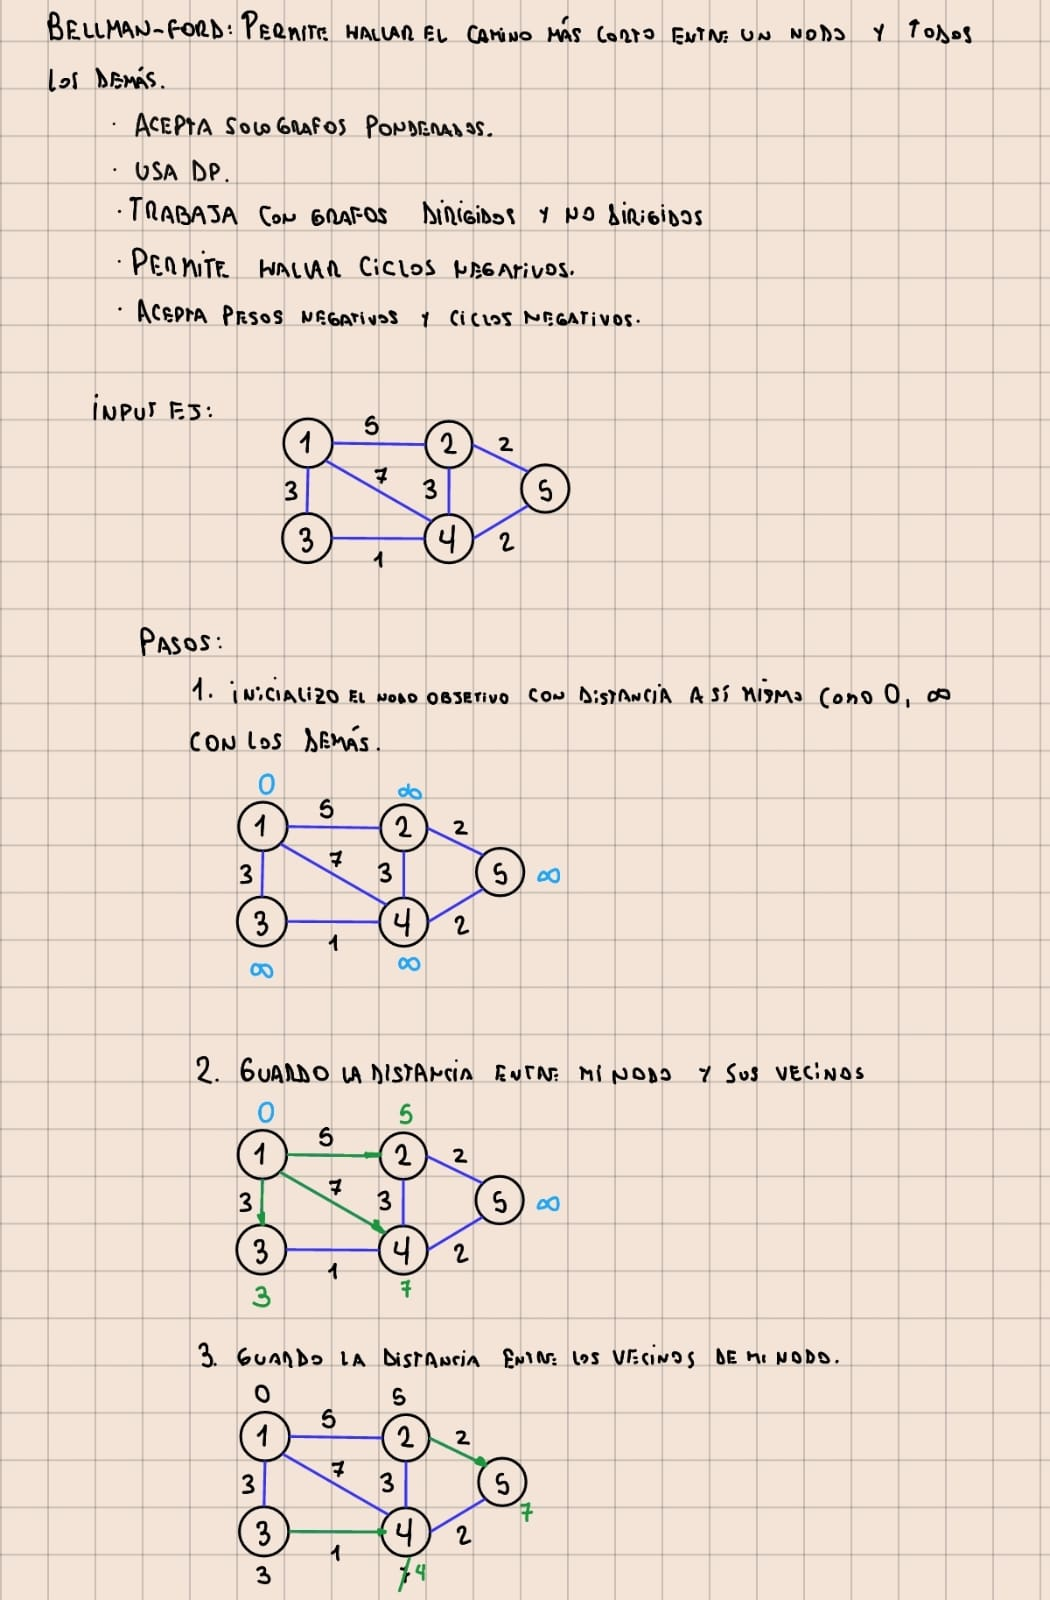
\includegraphics[width=\linewidth]{assets/bellman-ford-1.jpg}
\end{minipage}\]
\[\begin{minipage}[b]{0.8\textwidth}
    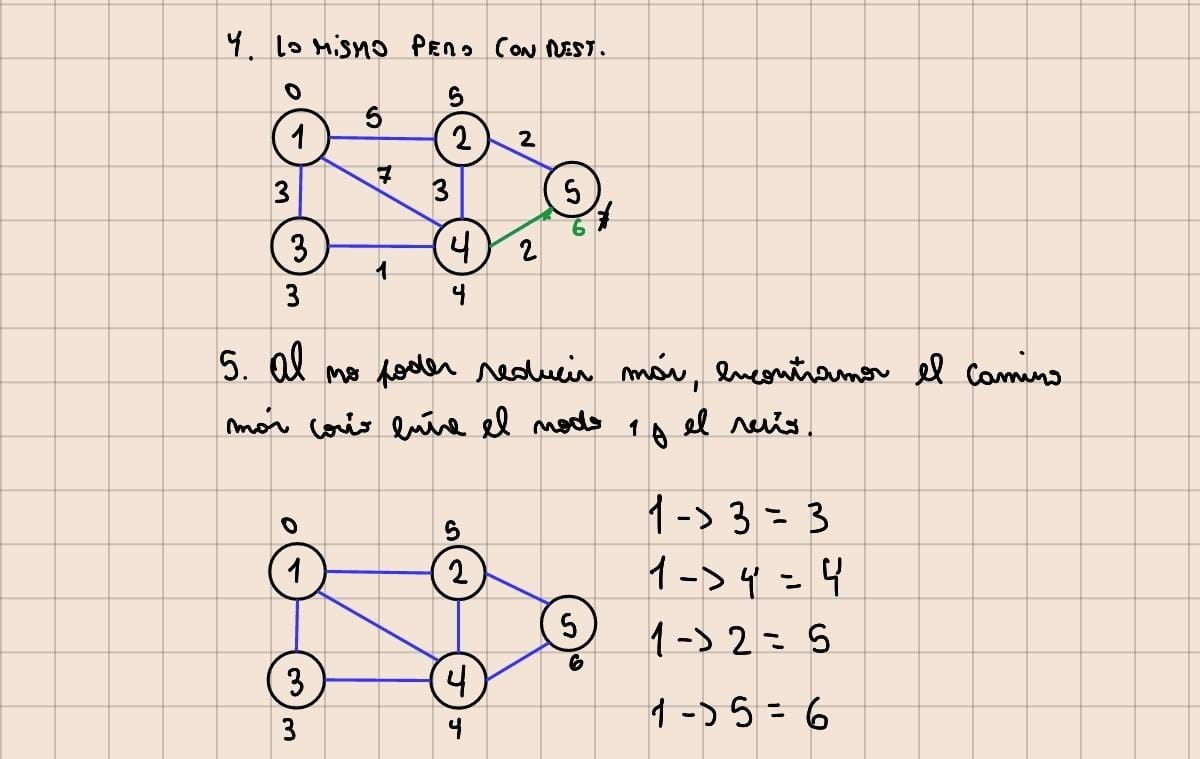
\includegraphics[width=\linewidth]{assets/bellman-ford-2.jpg}
\end{minipage}\]

\subsubsection*{All-Pairs-Shortest-Paths}
\textbf{Good to Know}: Es posible conseguir el mismo resultado haciendo $\longitud{V}$ operaciones pero con algoritmos de Single-Source-Shortest-Paths. ¿Vale la pena?, depende. Véase \hyperref[subsec:tradeoff_busqueda]{\textbf{Tradeoff entre Algoritmos de Búsqueda de Camino Mínimo}}
\subsubsection*{Floyd-Warshall (Técnica DP)}
Es un algoritmo que nos permite \textbf{en una sola operación} encontrar el \textbf{camino mínimo entre todos los pares de nodos} en un grafo ponderado. \\
Su implementación algorítmica es muy simple aunque este método es muy costoso dado que su complejidad temporal es $O(n^{3})$ y su complejidad espacial es $O(n^{2})$ que es el costo de armar la matriz. \\
¿Por qué tal complejidad temporal? Bueno... Porque se implementa con 3 for anidados. \\
Se basa en el uso de Programación Dinámica de forma bottom-up.
\subsubsection*{Requisitos de uso de Floyd-Warshall}
\begin{itemize}
    \item \textbf{Grafo ponderado}
    \item Puede trabajar con grafos dirigidos o no dirigidos 
    \item El grafo puede tener pesos negativos, pero no debe haber ciclos negativos
\end{itemize}
\subsubsection*{¿Cuándo usar Floyd-Warshall?}
\begin{itemize}
    \item Si necesitás todos los caminos más cortos entre \textbf{todos los pares de nodos}. Resuelve \textbf{muchos a muchos}.
    \item Si tenes pesos negativos pero no ciclos negativos (no es necesario tener pesos negativos)
    \item Puede trabajar con aristas de peso positivo o negativo.
    \item Cuando el grafo NO es demasiado grande.
\end{itemize}
\subsubsection*{Orden de operaciones}
\begin{itemize}
    \item Se arma una matriz, donde la distancia de todos los nodos a sí mismos es 0 (i = j => 0)
    \item Por cada nodo, se buscan las aristas que los conectan con los demás nodos, y se coloca en esa relación (ij), el peso de la arista.
    \item Se crean 3 for anidados. k, i, j que comienzan desde $i=1$ y van hasta la cantidad de nodos. 
    \item En cada iteración, se chequea que si la distancia actual de (ij) es mayor que agregando un nodo intermedio, entonces, la nueva distancia más corta es la de agregando ese nodo intermedio.
    \begin{itemize}
        \item Hay 2 casos que chequear al final.
        \begin{itemize}
            \item Si existía distancia inicial entre dos nodos y el valor final cambió, significa que se encontró un camino más corto.
            \item Si existía distancia inicial entre dos nodos y el valor final no cambió, significa que era el camino más corto.
            \item Si no existía distancia inicial $(\infty)$ y el valor final cambió, significa que se encontró un camino entre esos nodos.
            \item Si no existía distancia inicial $(\infty)$ y el valor final no cambió, significa que no se encontró un camino entre esos nodos.
        \end{itemize}
    \end{itemize}
\end{itemize}
Bocetos
\[\begin{minipage}[b]{0.7\textwidth}
    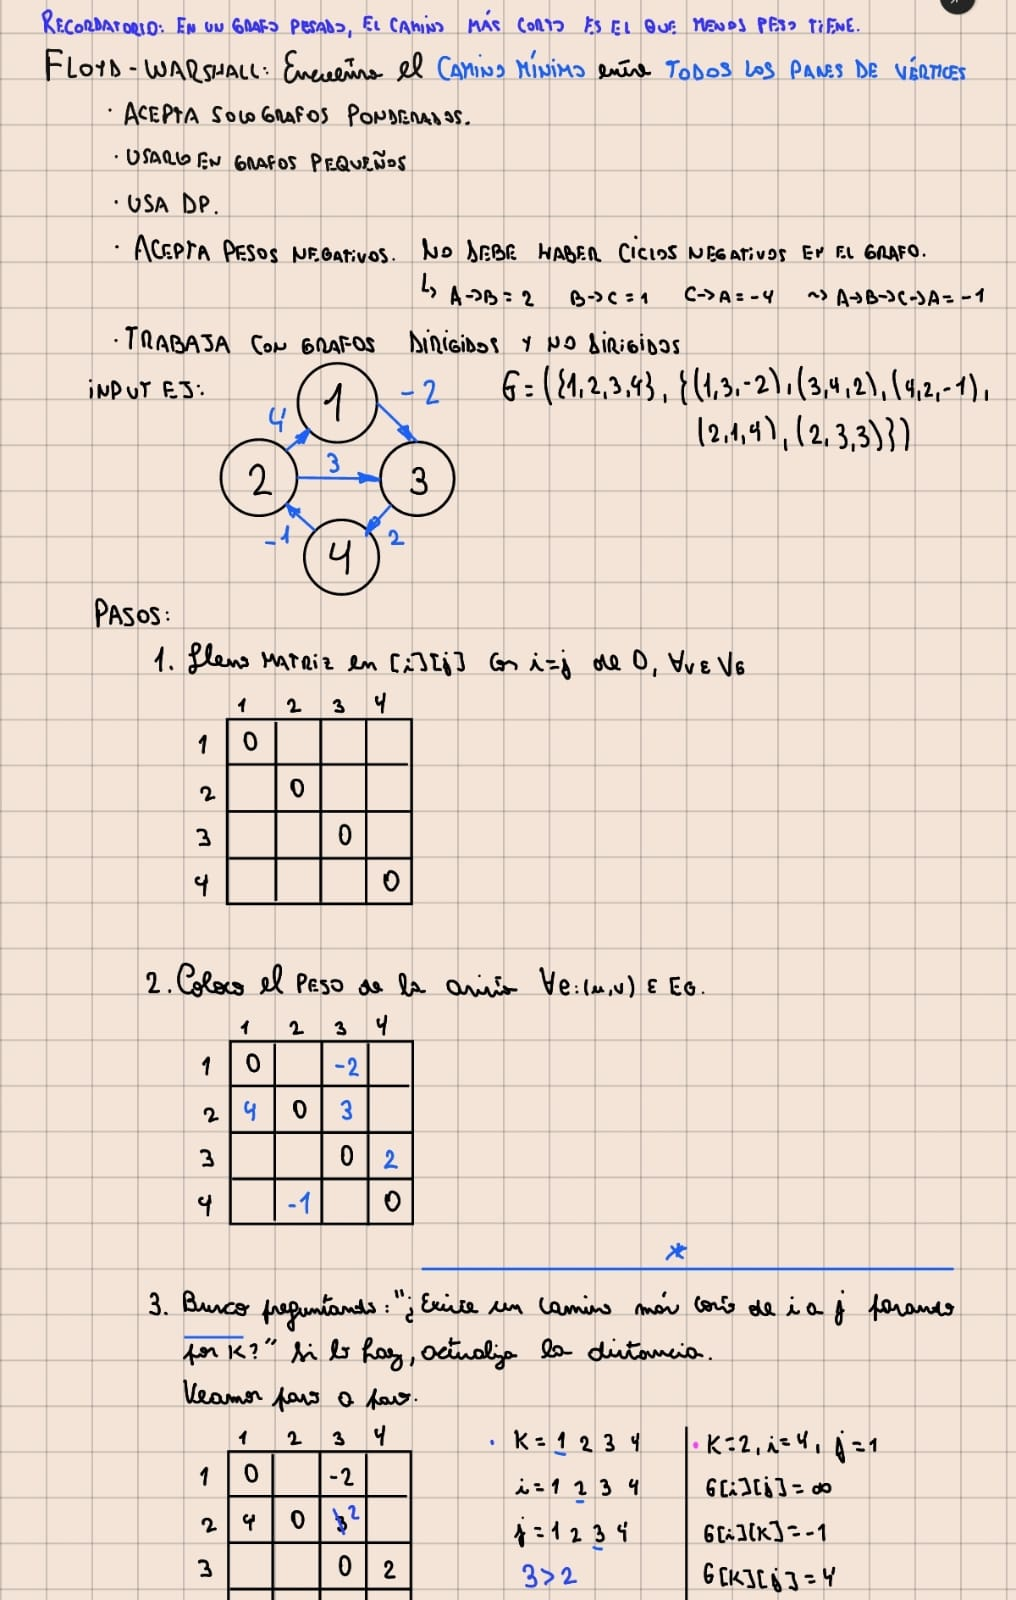
\includegraphics[width=\linewidth]{assets/floyd-warshall-1.jpg}
\end{minipage}\]
\[\begin{minipage}[b]{0.7\textwidth}
    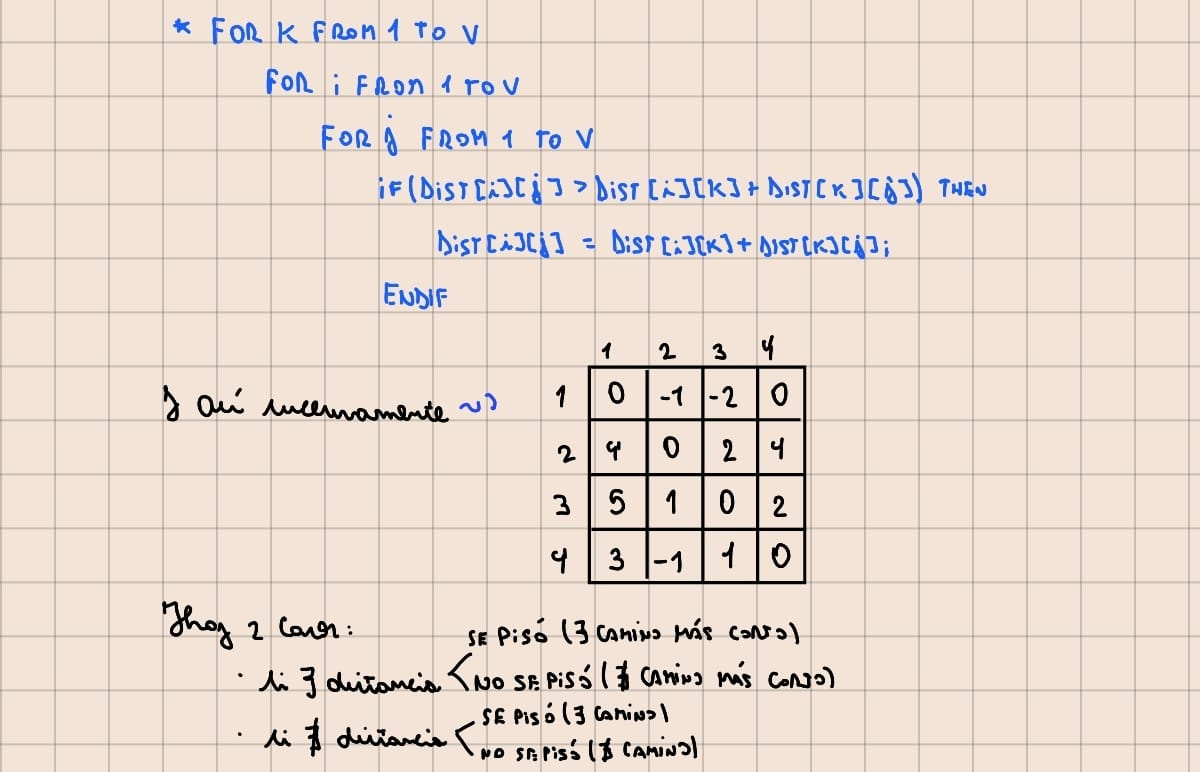
\includegraphics[width=\linewidth]{assets/floyd-warshall-2.jpg}
\end{minipage}\]
\subsubsection*{Algoritmo}
\begin{lstlisting}
    for (int i = 1; i <= n; i++) {
        for (int j = 1; j <= n; j++) {
            if (i == j) distance[i][j] = 0;
                else if (adj[i][j]) distance[i][j] = adj[i][j];
                else distance[i][j] = INF;
            }
    }

    for (int k = 1; k <= n; k++) {
        for (int i = 1; i <= n; i++) {
            for (int j = 1; j <= n; j++) {
                distance[i][j] = min(distance[i][j],
                distance[i][k]+distance[k][j]);
            }
        }
    }
\end{lstlisting}
\subsection*{Tradeoff entre Algoritmos de Búsqueda de Camino Mínimo}
\label{subsec:tradeoff_busqueda}
Es cierto que si tenemos un grafo pesado, podemos encontrar todas las relaciones de todos los nodos usando un método que sea \textbf{Single-Source Shortest Path}, resolviendo una vez por nodo, pero esto es muy ineficiente cuando tenemos un grafo grande. \\
No obstante, hay casos donde podría servir si no analizamos bien el problema. \\
Ej.: En \textbf{grafos dispersos}, sin \textbf{pesos negativos} es más óptimo usar implementaciones de Dijkstra (Min-Heap, Fibonacci Heap, etc.) $\longitud{V}$ veces antes que Floyd-Warshall. \\
Ej. 2: Tenemos un \textbf{grafo pesado acíclico} y aristas positivas. Queremos saber el \textbf{mínimo camino de un nodo a otros}. Si usamos Dijkstra la complejidad es \textbf{$O(V^{3})$} y Bellman-Ford es $O(V^{2}E)$. ¿Esto significa que Bellman-Ford es mejor? ¡No! Porque si el grafo fuese denso (no lo sabemos) entonces con Bellman-Ford la complejidad sería $O(V^{4})$
\subsubsection*{Topological Sort}
\label{subsubsec:topological_sort}
Topological Sort es un caso de uso real de DFS. Es un \textbf{ordenamiento lineal} de los nodos de un \textbf{grafo dirigido acíclico (DAG)} tal que, para cada arista $u \rightarrow v$, el nodo $u$ aparece antes que el nodo $v$. \\

Un orden topológico nos sirve para asegurarnos de \textbf{qué cosas deben cumplirse antes de que podamos hacer otras}. \\
Imaginemos que estamos creando un compilador, y tenemos muchos archivos que dependen de diversas librerías. Por ejemplo, una de las librerías es \textbf{Pow}, que depende de \textbf{Math}, y \textbf{Main} también necesita de \textbf{Math} para funcionar correctamente. \\
En este caso, tenemos dos dependencias claras:
\begin{itemize}
    \item \textbf{Pow} no funciona sin \textbf{Math}, porque depende de funciones dentro de esa librería. Por lo tanto, primero tenemos que compilar \textbf{Math} antes de poder acceder a \textbf{Pow}.
    \item \textbf{Main} no funciona sin \textbf{Math}, porque necesita funciones de allí. Así que también tenemos que compilar \textbf{Math} antes de poder acceder a \textbf{Main}.
\end{itemize}
\textbf{¿Qué tiene que ver esto con grafos?} Bueno, podemos tratar a las entidades (\textbf{Pow}, \textbf{Math} y \textbf{Main}) como nodos, y las dependencias entre ellas como aristas del grafo. Es decir:
\[
V = \{ \text{Pow}, \text{Math}, \text{Main} \}, \quad E = \{ (\text{Math}, \text{Main}), (\text{Math}, \text{Pow}) \}
\]

Ahora viene la parte interesante: el \textbf{ordenamiento topológico}. ¿Dónde está? La idea es que podemos cambiar el orden de los nodos siempre y cuando respetemos el orden de las dependencias. Es decir, \textbf{Main} no puede ser compilado antes de \textbf{Math}. Sin embargo, no importa si \textbf{Pow} o \textbf{Main} se compilan antes de lo otro, siempre y cuando \textbf{Math} esté compilado primero. \\
Por lo tanto, tenemos dos posibles representaciones topológicas del problema:
\begin{itemize}
    \item $ \text{Math} \rightarrow \text{Pow} \rightarrow \text{Main} $
    \item $ \text{Math} \rightarrow \text{Main} \rightarrow \text{Pow} $
\end{itemize}
Ambas cumplen con la condición de que \textbf{Math} debe compilar antes que \textbf{Pow} y \textbf{Main}, pero no importa si \textbf{Pow} o \textbf{Main} se compilan antes que el otro. \\
¿Qué pasa si las dependencias cambian? Imaginemos el siguiente conjunto de dependencias:
\[
V = \{ \text{Pow}, \text{Math}, \text{Main} \}, \quad E = \{ (\text{Math}, \text{Main}), (\text{Math}, \text{Pow}), (\text{Pow}, \text{Main}) \}
\]
En este caso, solo existe \textbf{un único orden topológico válido}:
\begin{itemize}
    \item $ \text{Math} \rightarrow \text{Pow} \rightarrow \text{Main} $
\end{itemize}
Esto es porque la arista $(\text{Pow}, \text{Main})$ obliga a que \textbf{Pow} se compile antes que \textbf{Main}, eliminando las opciones de reordenar \textbf{Pow} y \textbf{Main}. \\
\textbf{¿Para qué me sirve esto?} Para asegurarnos de que no hay \textbf{dependencias cíclicas} y que todas las dependencias se resuelven en el orden correcto, manteniendo la integridad de las relaciones entre las entidades. \\
\textbf{Implementación con DFS}: 
\begin{lstlisting}
    topoSort(graph G)
        for each vertex u in V[G] do
            state[u] = UNVISITED
            parent[u] = NULL
        end for
        time = 0
        for each vertex u in V[G] do
            if state[u] = UNVISITED then
                TOP_VISIT(u)
            end if
        end for
    end function
\end{lstlisting}
\textbf{Good to Know}: Si existen varios nodos que no tienen dependencias entre sí, hay más de una forma válida de realizar el orden topológico. En estos casos, el orden en que aparecen esos nodos no tiene importancia, y puedes elegir su disposición según tus preferencias al implementar el algoritmo. El orden topológico solo se asegura de que los nodos con dependencias se ubiquen en el orden correcto, pero no especifica el orden de los nodos independientes. \\
La complejidad es la misma que DFS, $\theta(\longitud{V} + \longitud{E})$
\section*{Fuerza Bruta}
Consiste en analizar y listar todas las posibilidades y quedarme con las que me interesan. \\
En la fuerza bruta, existen problemas de factibilidad y optimalidad. 
\begin{itemize}
    \item En los problemas de factibilidad lo que queremos son soluciones que cumplan ciertas características. 
    \item En los problemas de optimizaciones combinatorias, teniendo todas las soluciones factibles me quedo con la mejor (según el criterio que considero qué es mejor). 
\end{itemize}
Los algoritmos por fuerza bruta son muy fáciles de implementar pero son muy ineficientes; son útiles cuando tenemos instancias súmamente pequeñas. \\
Ej.: Si tenemos que completar un tablero de ajedrez tendríamos que poner todas las posibilidades en todos los casilleros y si hay pocas soluciones válidas estaríamos tardando demasiado tiempo por nada.
\section*{Backtracking}
Es una modificación de la técnica de fuerza bruta que aprovecha propiedades del problema para evitar analizar todas las configuraciones. \\
Para que el algoritmo sea correcto debemos estar seguros de no dejar de examinar configuraciones que estamos buscando. \\
Las soluciones candidatas se representan con un \textbf{vector a = $(a_{1}, a_{2}, \dots, a_{n})$}
\begin{itemize}
    \item Soluciones parciales: Son las soluciones que se van armando en cada paso. 
    \begin{itemize}
        \item Cada nodo es una solución parcial.
        \item La raíz del árbol es el vector vacío (solución parcial vacía).
    \end{itemize}
    \item Soluciones candidatas: Depende el problema. A veces son todas las hojas (si necesitás gastar todos los elementos), a veces te basta con cumplir X cosa y no necesitás recorrer todo el árbol. 
    \item Soluciones válidas: Son aquellas soluciones que cumplen con todas las características que buscamos. A veces son las hojas del árbol, a veces no es necesario llegar hasta las hojas, porque capaz se cumple en uno, o dos pasos tempranos.
\end{itemize}
\textbf{¿Todas las soluciones candidatas son soluciones parciales? Porque si una posible solución válida llegás en el primer nivel del árbol, entonces esa solución era candidata, pero también era parcial.} \\
Ej.: Ejercicio de armar subconjuntos que sumen n.  
\subsection*{Podas}
En el backtracking, recorremos el árbol en profundidad. \\
Cuando podemos ver que una solución parcial no nos llevará a una solución válida, no es necesario seguir explorando esa rama del árbol de búsqueda (se poda el árbol) y se retrocede hasta encontrar un vértice con un hijo válida por donde seguir. 
\begin{itemize}
    \item Poda por factibilidad: Ninguna extensión de la solución parcial derivará en una solución valida del problema. 
    \begin{itemize}
        \item Digamos que quiero llegar a armar subconjuntos que sumen 9, si con el nodo actual la suma es 10, entonces no me sirve seguir hacia adelante. Podo de una. Esto se llama \textbf{propiedad dominó}, si una solución parcial no vale, la generada a partir de ella menos todavía. 
        \item \textbf{¿Qué pasaría, si llegase a haber algún caso donde capaz nuestra solución parcial ya no es válida, pero si seguíamos adelante capaz teníamos un factor que la volvía a hacer válida? Por ej.: En un conjunto que tenes números positivos y negativos tenés que armar subconjuntos que sumen k. Si te pasaste de k, no te sirve podar de una porque capaz encontrás algun negativo que te ayude a llegar a k de vuelta.}. Respuesta: No te sirve esa poda para ese problema. 
    \end{itemize}
    \item Poda por optimalidad (problemas de optimización): Ninguna extensión de la solución parcial derivará en una solución del problema óptima.
\end{itemize}
Un problema de backtracking que no tiene podas es un problema de fuerza bruta.
\subsection*{Correctitud en Backtracking}
Para demostrar la correctitud de un algoritmo de backtracking, debemos demostrar que se enumeran todas las configuraciones válidas. Si hacés una poda, me tenés que garantizar que aunque el rendimiento haya mejorado, me sigas trayendo las mismas soluciones válidas. \\
Ej.: Si lo hacemos por fuerza bruta, podemos conseguir todas las soluciones válidas. Luego, si lo hacemos por backtracking y añadimos podas, nos fijamos que tengamos los mismos resultados que si lo hacemos por fuerza bruta.
\subsection*{Complejidad en Backtracking}
Consideramos el costo de procesar cada nodo. Cada nodo aparece cada vez que hacemos un llamado recursivo.  
\subsection*{Tips Backtracking}
\begin{itemize}
    \item Si tengo conjuntos, solo me interesan tener una única ocurrencia. Es decir, $\{1, 3\} = \{3, 1\}$ por lo tanto, siempre priorizo que el elemento de la izquierda pueda tener a todos los mayores de la derecha pero no al revés. Esto gana mucho tiempo porque estamos eliminando soluciones repetidas.
    \[\begin{minipage}[b]{0.9\textwidth}
    \includegraphics[width=\linewidth]{assets/backtracking_half_search.png}
    \end{minipage}\]
\end{itemize}
\section*{Programación Dinámica (DP)}
Se basa en solucionar y memorizar subproblemas que se repetirán para ahorrar tiempo. \\
Esa \textbf{superposición de problemas} es que estamos llamando usando algo que \textbf{ya resolvimos anteriormente}, entonces, para evitar calcular todo nuevamente, usamos la información almacenada en memoria. \\
Es \textbf{bastante común} usar este tipo de estrategias para afrontar problemas con matrices, o casos recursivos para cosas altamente costosas de calcular. \\
\textbf{Importante}: ¿Cuándo hay veces que la entrada no es exactamente igual pero vale la memorización para ese subproblema? \\
Cuando la dirección de los argumentos no importa, se puede utilizar ese subproblema memorizado, es decir, en casos donde, por ejemplo $(a, b) = (b, a)$.
\subsection*{Propiedades de la Programación Dinámica}
Existen varios conceptos importantes que debemos tener en cuenta para entender el uso de programación dinámica:
\begin{itemize}
    \item Estado: Representa una subparte del problema original. Se define por las variables mínimas necesarias para describir un subproblema.
    \item Caso base: Es la condición inicial del problema. Define cuándo detener la recursión y que valor devolver en ese caso.
    \item Caso recursivo: Es la definición del problema en función de subproblemas más pequeños. 
    \item Transición: Es la regla que te lleva de un estado a otro, es decir, cómo se construye una solución a partir de otras. Qué hacés con el llamado recursivo.
    \item Orden Topológico: Es el orden obligatorio con que se realizan las operaciones.

\end{itemize}
Veamos un ejemplo de un código real para categorizar los ítems anteriormente mencionados
\begin{lstlisting}
    long long fibo(int n, std::vector<long long>& memo){ //Estado: n, es lo que importa para memorizar.
    if(memo[n] != 0) return memo[n];
    
    if(n == 0) return 0; // Caso base 
    if(n == 1) return 1; // Caso base

    auto state1 = fibo(n-1, memo); //Caso recursivo
    auto state2 = fibo(n-2, memo); //Caso recursivo
    memo[n] = state1 + state2;  //Transición
    return memo[n];

    Orden topológico: calcular fibo(0), luego fibo(1), luego fibo(2), luego fibo(3), ... etc.
    
    DAG: Una cadena de dependencias 0 -> 1 -> 2 ... -> n (como resuelve en base al param n)

    }
\end{lstlisting} 
Veamos unos ejemplos más
\begin{lstlisting}
    vector<long long> fact(n+1, 1);
    vector<long long> sum(n+1, 0);
    for(int i=1; i<=n; ++i){
        fact[i] = i * fact[i-1];
        sum[i] = sum[i-1] + fact[i];
    }
    return sum[n];

    Transición:
        fact[i] = i * fact[i-1];
        sum[i] = sum[i-1] + fact[i];
    (como sum[n] es la respuesta, y sum[i] depende de sum y fact, eso cambia el estado).
    
        Orden topológico: primero calculo fact[0..n], y luego sum[0..n].
    
    DAG: fact[0] -> sum[0] -> fact[1] -> sum[1] -> fact[2] -> sum[2] ... -> fact[n] -> sum[n]
\end{lstlisting}
\begin{lstlisting}
    
\end{lstlisting}

\subsection*{Formas de realizar programación dinámica}
Se puede hacer tanto de forma Top-Down (recursivamente) o Bottom-Up (iterativamente). \\
En Top-Down hablamos de \textbf{memorización} mientras que en Bottom-Up hablamos de \textbf{tabulación}. 
\subsubsection*{Bottom-Up vs Top-Down}
\begin{itemize}
    \item Top Down (memorización): Usamos recursión, guardamos los resultados en una caché (generalmente diccionario o array). Solo resolvemos los subproblemas que necesitamos. Normalmente, en espacio, ya ocupa O(n) por la profundidad del stack. Cada llamado recursivo ocupa O(n). 
    \item Bottom Up (tabulación): Usamos un enfoque iterativo, contruimos la solución desde los casos base hacia arriba mientras que llenamos una tabla paso a paso. 
\end{itemize}
\[\begin{minipage}[b]{0.8\textwidth}
    \includegraphics[width=\linewidth]{assets/topdown_bottomup.png}
\end{minipage}\]
\subsection*{Programación Dinámica Top-Down}
\subsubsection*{Fibonacci y su relación con la Programación Dinámica}
\[\begin{minipage}[b]{0.8\textwidth}
    \includegraphics[width=\linewidth]{assets/fib_dp.png}
\end{minipage}\]
¿Donde está la superposición de problemas acá? Bueno, veamos que para \textbf{fib 5} se encuentra repetida una vez. \\
Entonces, la idea, es que guardemos el resultado para el primer \textbf{fib} que salga, y luego reutilizarla. \\
Nótese que al ser \textbf{fib(n-1)} + \textbf{fib(n-2)} en algún momento, indudablemente el \textbf{n-1} va a llegar a ser el valor que fue \textbf{n-2}, y ahí justamente, entra la memorización. \\
A nivel código, no es más que guardar en un array, map o una estructura eficiente. \\ 
Sin ningún tipo de memorización, la complejidad que da en tiempo es $O(n^{2})$ mientras que en espacio da $O(n)$. \\
\textbf{En espacio da $O(n)$} porque a nivel stack, lo más profundo que baja en una rama es n veces. 
\subsubsection*{Con Programación Dinámica}
Sabiendo que tenemos superposición de problemas basado en n, optimizado quedaría así
\[\begin{minipage}[b]{0.9\textwidth}
    \includegraphics[width=\linewidth]{assets/fib_dp_finish.png}
\end{minipage}\]
¿Cómo quedó la complejidad temporal y espacial? Bueno, espacialmente seguimos teniendo $O(n)$ porque bajamos hasta el caso base, al menos una vez, pero temporalmente ahora también tenemos $O(n)$
\[\begin{minipage}[b]{0.9\textwidth}
    \includegraphics[width=\linewidth]{assets/fib_dp_finish_o.png}
\end{minipage}\]
\subsubsection*{Llegando a un punto particular en una grilla}
Digamos que queremos movernos a un punto particular fijo y solo podemos movernos a la derecha y para abajo. Es sabido que van a existir muchas formas de llegar a ese punto. \\
Ahora bien, a medida que nos vamos acercando, el problema se achica. Así que, seguramente, vaya a existir algún otro camino por el que lleguemos al punto (o no). 
\[\begin{minipage}[b]{0.9\textwidth}
    \includegraphics[width=\linewidth]{assets/gridTraveler.png}
\end{minipage}\]
Sin ningún tipo de memorización, la complejidad que da en tiempo es $O(2^{n+m})$ porque para cada caso, tengo dos opciones que dependen de dos variables mientras que en complejidad espacial da $O(n+m)$ que es lo que nos cuesta bajar hasta el caso base gastando todas las opciones.
\subsubsection*{Con Programación Dinámica}
¿Cómo hacemos para guardar en una estructura de memorización algo que tiene más de un argumento? Normalmente, lo ideal es guardar algo de la especie \textbf{m + ', ' + n}. \\
Es realmente importante NO guardar todos de forma continua y sí distinguirlos por algún símbolo \textbf{(,)} por si en algún momento, tenemos que considerar los elementos separados pero que valgan por simetría.
\[\begin{minipage}[b]{0.9\textwidth}
    \includegraphics[width=\linewidth]{assets/gridTraveler_2.png}
\end{minipage}\]
Por último, veamos como mejoró nuestra solución\[\begin{minipage}[b]{0.9\textwidth}
    \includegraphics[width=\linewidth]{assets/grid_traveler_op.png}
\end{minipage}\]
\subsubsection*{Receta de Programación Dinámica (Top-Down)}
\begin{itemize}
    \item Hacer que la solución sin programación dinámica funcione
    \begin{itemize}
        \item Visualizar el problema como un árbol.
        \item Implementar ese árbol usando recursión.
        \item Testear si la solución funciona. 
    \end{itemize}
    \item Optimizarlo
    \begin{itemize}
        \item Agregar un objeto de memo.
        \item El objeto memo debe pasarse a todos los llamados recursivos. Normalmente lo pasamos por referencia o usamos variables globales.
        \item Agregar casos base para los valores memorizados.
        \item Guardar los valores de los return dentro del objeto memo.
    \end{itemize}
\end{itemize}
Para resolver problemas de programación dinámica se recomienda ser meticuloso, hacer dibujos, armar buenas soluciones de fuerza bruta y recién luego pensar la estrategia de memorización. Memorizar es sencillo, qué memorizar es complicado. \\
No traten de implementar una solución óptima desde el principio. Make it work first.
\subsubsection*{canSum problem}
La idea es que dado un array, se diga si existe algún subconjunto de elementos que suman un valor n particular. \\
\textbf{Tip importante}: En problemas donde hay que llegar a determinado valor k, siempre, pero siempre conviene disminuir ese valor de target y no ir sumando.
\[\begin{minipage}[b]{1\textwidth}
    \includegraphics[width=\linewidth]{assets/canSum.png}
\end{minipage}\]
Algo que siempre hay que tener en cuenta es que, si llegamos a determinado valor, el árbol siempre va a tener el mismo comportamiento para ese valor. Nótese que acá, en este problema particular tampoco nos interesa qué numeros suman nuestro target, sino, simplemente si hay un camino o no.
\subsection*{Programación Dinámica Bottom-Up}
\subsection*{Demostraciones por Construcción}
En grafos, las demostraciones por construcción funcionan exhibiendo un ejemplo de que se cumplen todas las cosas que nos piden y, a veces (si se nos pide) demostramos unicidad. \\
Si la unicidad es necesaria, normalmente, suelen estar relacionadas con hablar de isomorfismo de grafos, es decir, que quizá existe algún otro grafo pero es un isomorfo del original. \\
Eso quiere decir que podríamos transformar un grafo a otro a través de una función y teóricamente sería el mismo, solo que cambia el nombre de algún vértice. \\
Ej.: Demostrar en forma constructiva que para cada n existe un \textbf{único} grafo orientado \textbf{cuyos vértices tienen todos grados de salida distintos}. Un grafo orientado es un grafo donde todos sus aristas tienen una orientación pero existe al menos una arista que no es simétrica. \\
Si todos los vértices tienen grados de salida distintos significa que si tenemos n vértices, tenemos n-1 grados de salida diferentes. \\
Necesitamos un vértice con grado de salida 0, otro con grado de salida 1, otro con grado de salida 2, etc, etc. \\
Entonces la idea es que a mayor n, ese se conecte con todos los \textbf{anteriores}. \\
Es decir, dout(1) = 0, dout(2) = 1, dout(3) = 2, etc, etc. \\
Entonces ahora sí hagamos la demostración: Sea G = (V, E) un grafo cuyos vértices tienen grados de salida distintos, y existe al menos una arista que no es simétrica. \\
Definimos $ V = \{V_{1}, V_{2}, V_{3}, ..., V_{n}\}$ como los vértices de nuestro grafo donde le asignaremos los grados de salida de la siguiente manera: $dout(V_{1}) = 0, dout(V_{2}) = 1, \dots, dout(V_{n}) = n-1$ \\
Luego, las aristas que tendremos en E serán de la forma $e = (V_{i}, V_{j})$ donde si existe e no existirá $e' = (V_{j}, V_{i})$. De lo contrario, podría suceder que no todos los vértices tengan grados de salida diferentes. \\
Finalmente, este grafo es único porque existe una única forma de conectar los vértices del grafo para que tengan grados de salida diferentes y esto funciona sin colocar simetrías entre las aristas, y también existe una única forma de asignar n grados diferentes entre n vértices. \\
Finalmente, si existe otro grafo, es un isomorfo de este, es decir, quizá cambian los nombres de los vértices pero la cantidad de aristas es la misma. \\
\section*{Anexo}
\subsection*{Demostraciones de Grafos}
Normalmente se hace inducción sobre las aristas, aunque en algunos casos, optamos sobre los vértices. \\
Lo más común es tener un caso base del tipo $n=1, m=0$ o $n=2, m=1$. \\
\textbf{Good to Know}: Usar a favor las propiedades.
\subsubsection*{Distancia entre dos vértices}
\label{subsubsec:distancia_demostracion}
Si P es el recorrido entre u y v tiene longitud d(u,v) $\implies$ P es un camino. \\
Recordemos algunas definiciones
\begin{itemize}
    \item Un recorrido es una sucesión de vértices y aristas, que no tiene ninguna limitación.
    \item d(u, v) es el recorrido más corto entre u y v. Por lo que, podría haber otros. 
    \item P es un camino: Un camino es un subconjunto de un recorrido donde no puede haber vértices repetidos.
\end{itemize}
Probando por el absurdo: 
\[\neg Q \implies R\]
En este caso
\begin{itemize}
    \item $\neg Q$ = P no es un camino
    \item $R$ = P es el recorrido entre u y v y tiene longitud d(u,v)
\end{itemize}
La idea es llegar a algo falso.  
\[V \implies F = F\]
Suponemos que P NO es un camino $\neg Q = V$, entonces hay, al menos un vértice en P que se repite.  \\
Recorrido P \[u \rightarrow z \rightarrow z \rightarrow v\]
¿Podemos encontrar algún camino que sea más corto que P? (esto haría falso el consecuente). \\
Defino un camino T \[u \rightarrow z \rightarrow v\] 
Luego, la distancia mínima entre ambos recorridos
\[min(dP(u,v), dT(u,v)) = min(3, 2) = 2 = dT(u,v)\]
Finalmente, llegamos a un absurdo, porque la distancia mínima la tenemos con el recorrido T y no con P. \\
Si hubiesemos llegado a que con $\neg Q$, P es el camino más corto, hicimos mal la demostración.
\subsection*{Representación de grafos en la práctica}
\label{subsec:representacion_grafos_practica}
\textbf{Resumen}: Si el grafo es denso $\longitud{E}$ es igual de grande que $\longitud{V}^{2}$ y necesitás saber si existe una arista entre dos vértices lo más rápido posible, usá una matriz de adyacencia. Caso contrario, una lista de adyacencia. 

\subsubsection*{Numeración de los vértices}
Numeramos los vértices desde 0 hasta n-1 (donde n es la cantidad de vértices). Esto hace que sea más fácil de trabajar con arrays y matrices.

\subsection*{Ejemplo}
Queremos ver si podemos llegar desde la ciudad A hasta la ciudad D. Un cliente nos trae la siguiente información donde la primer letra corresponde al saliente y la segunda el destino. \\
\begin{lstlisting}
{
  "rutas": [
    ["A", "B"],
    ["B", "C"],
    ["C", "D"],
    ["A", "E"],
    ["E", "F"]
  ],
  "origen": "A",
  "destino": "D"
}
\end{lstlisting}
Acá es donde tenemos que pensar cómo armamos nuestro grafo. 
\subsubsection*{Forma 1 (Lista de Adyacencia)}
Sabemos que tenemos que ir desde una ciudad a otra, asì que estarìa bueno tener la lista de conexiones de una ciudad con todas las demás. Es decir, meter todas las ciudades con las que se conecta una en una lista. \\
En este caso, nos conviene una lista de adyacencia (conjunto vecindario) y ahora veremos por qué.\\
Nos quedaría entonces, algo así 
\begin{lstlisting}
    graph = {
        "A": ["B", "E"],
        "B: ["C"],
        "C": ["D"],
        "E": ["F"],
    }
\end{lstlisting}
El problema entonces sería algo así: 
\begin{itemize}
    \item Empiezo en A, tomo cada vecino de él y me fijo con quién se conectan.
    \begin{itemize}
        \item Llegué a B
        \begin{itemize}
            \item B se conecta con C, C se conecta con D, entonces A se conecta con D. 
            \item B se conecta con E, E se conecta con F y F no se conecta con nadie.
        \end{itemize}
        \item Respuesta final: Sí existe un camino, y ese es A -> B -> C -> D y es un circuito simple.
    \end{itemize}
\end{itemize}
¿Cómo quedaría de esta manera, la complejidad temporal y espacial en el armado del grafo? 
\begin{itemize}
    \item Temporal:O(E) porque el input inicial es una lista de aristas y recorremos toda esa lista.
    \item Espacial: O(V + E) porque por cada nodo, guardamos una lista de sus vecinos.
\end{itemize}
¿Y en la búsqueda? 
\begin{itemize}
    \item Espacial: O(V) que es lo que cuesta ir guardando los nodos visitados. 
    \item Temporal: O(V + E) porque por cada nodo, vemos todas sus aristas.
\end{itemize}
¿Cuál es la complejidad total del algoritmo? En tiempo es O(V + E) y en espacio O(V + E). \\
\textbf{¿Cuando usar listas de adyacencias?}
\begin{itemize}
    \item El grafo es disperso, es decir, tiene más aristas que nodos.
    \item Es importante optimizar el espacio.
    \item Buscás los vecinos frecuentemente.
\end{itemize}
\subsubsection*{Forma 2 (Matriz)}
Es importante recordar que en la matriz, la dimensión es siempre como si todos los nodos estarían relacionados con todos. \\
En este caso tenemos 6 nodos, y en el peor caso se conectan todos con todos. Así que la matriz sería de 6x6. \\
\begin{lstlisting}
    matrix = [
    [0, 1, 0, 0, 1, 0],  //A
    [0, 0, 1, 0, 0, 0],  //B
    [0, 0, 0, 1, 0, 0],  //C
    [0, 0, 0, 0, 0, 0],  //D
    [0, 0, 0, 0, 0, 1],  //E 
    [0, 0, 0, 0, 0, 0],  //F 
]
\end{lstlisting}
¿Cómo quedaría de esta manera, la complejidad temporal y espacial en el armado del grafo? 
\begin{itemize}
    \item Temporal: O($V^{2}$).
    \item Espacial: O($V^{2}$).
\end{itemize}
¿Y en la búsqueda? 
\begin{itemize}
    \item Buscar todos los vecinos de A - Tiempo: O(V).
    \begin{itemize}
        \item Buscar todos los vecinos B - Tiempo: O(V). Buscar todos los vecinos de C - Tiempo: O(V). 
        \item Buscar todos los vecinos de E - Tiempo: O(V). Buscar todos los vecinos de F - Tiempo: O(V).
    \end{itemize}
\end{itemize}
Como esto se hace varias veces, sería algo de O(cantVecinosNodo * V) = O(V). \\
¿Cuál es la complejidad total del algoritmo? En tiempo y espacio es O($V^{2}$). \\
\textbf{¿Cuando usar matrices de adyacencia?}
\begin{itemize}
    \item El grafo es denso ($\longitud{E} \approx \longitud{V}^{2}$).
    \item Necesitás verificar si existe rápidamente una conexión entre dos nodos.
    \item El grafo es estático, es decir, no se agregan ni se quitan aristas frecuentemente.
\end{itemize}
\subsubsection*{Comparación de las dos estructuras}
\begin{table}[h!]
    \centering
    \begin{tabular}{|l|c|c|}
    \hline
    \textbf{Operación}                        & \textbf{Lista de Adyacencia}          & \textbf{Matriz de Adyacencia}      \\ \hline
    \textbf{Espacio (Construcción)}           & O(N + E)                             & O(N²)                              \\ \hline
    \textbf{Tiempo (Construcción)}            & O(N + E)                             & O(E)                               \\ \hline
    \textbf{Acceder a los Vecinos (por Nodo)} & O(1)                                 & O(N)                               \\ \hline
    \textbf{Tiempo para Buscar Camino}        & O(N + E) (DFS/BFS)                   & O(N²)                              \\ \hline
    \textbf{Espacio Temporal (Búsqueda)}      & O(N)                                 & O(N)                               \\ \hline
    \textbf{Acceder a la existencia de una Arista} & O(k) (conjunto de vecinos)    & O(1)                               \\ \hline
    \end{tabular}
    \caption{Comparativa de complejidad temporal y espacial de las representaciones de grafos.}
\end{table}

\end{document} 

